\chapter{NOTEBOOKS FROM TRASHED PAPERS}


% başka bir yerde kullanırsın: , as illustrated by the examples cited so far,


% Epigraph
\begin{singlespace}
% FROM Wild Art. quote taken from the television series `American Masters', Season 5, Episode 8, John Cage: I have nothing to say and I am saying it (aired on 17 September 1990).
\epigraph{The first question I ask myself when something doesn't seem to be beautiful is why do I think it's not beautiful? And very shortly you discover that there is no reason. If we can conquer that dislike, or begin to like what we did dislike, then the world is more open. That path ---of increasing one's enjoyment of life--- is the path, I think, we all best take: to use art not as self-expression, but as self-alteration; to become more open.}{\hfill---John Cage, \textit{Wild Art}, 2013}
\end{singlespace}





In this chapter thesis project and its development progress will be explained in detail in the light of what has been discussed in previous chapters. The project will be examined in various dimensions. The relationship will be established between the previously mentioned artworks. How this project is related to the discussed concepts and how it can be positioned among the previous works will be explained.

Firstly, brief statement and description of the work is given. Secondly, the development of the project and experiments are explained. Lastly, the final body of the work with its parts is presented.





%
%
% TODO: Burada geçmiş, şimdiki zamanlara dikkat etmek gerek.
\section{The Statement}
% TODO Ekolojik, harmful, iğreç falan diye de değinmek gerekli bence.
% --disgusting, abject, unattractive, harmful to the people and nature--
Refuse is part of people’s consumption practices. It is a very common concept from developed cities to rural areas, from modern societies to ancient societies. It is not wanted, thrown away, kept away. It is considered as useless and disgusting. Contrary to the common approach as \cite{thompson1979rubbish}, author of the book Rubbish Theory, stated \quotes{one man's trash is another man's treasure}.

% Her zaman her yerde olan çöp.
% people are invited in the phase of collecting and finding trash
With the collaboration of many people discarded papers and packages were collected from different places. This time, it was not thrown away, it was collected and saved. Later they were transformed to notebooks by hand with traditional methods. Juxtaposition of trashes create notebooks that are different from the blank industrial ones, and through them challenged the widespread understanding of trash.

Through this project trash were re-imagined (re-considered, re-thought), new possibilities and alternatives were seek. As it is discarded, missed potentials were discovered. 

The purpose is not to build an object that is produced from discarded material to watch it from distance. The important thing is to interact with it. It is already discarded and general behavior avoid from it. This work must change it. It must call the viewer to interact with it. Trash must be accepted by them. For this reason notebooks are given away free at various places where people visit frequently. By doing that once thrown materials would find a place with new purposes in the community.

% Bu proje çöpte yeni imkanlar bulmayı amaçlıyor. İnsanların tekrar onları hayatlarına sokmalarını istiyor.





%
%
\section{Development Progress of the Project}
In order to have an insight of this project and realize artistic intentions, it is important to look at the process that reveals the path to the final work and critical decisions that were necessary to the completion of the project.

% Starting from the very beginning, I would like to explain which paths and turns I took and how they let my work to come out as it is now. In other words, this will be the story of how I developed my work from scratch.

% Artist's work and their approach supported my project.
Through the process, there are several problems that needed to be solved. Some of the questions in my mind are solved through the research on trash. Further, the found samples of artworks helped me a lot to shape unclear points of the project. They provide me a deeper understanding of the subject and what I am doing. They lead me during the development of the work.
% played significant role.
% It is evolved in time and affected from other artists' work, and gain meaning from research.

% This progress also reveals the how this work can be positioned among the other works.







% NEW PART [approach, history] 
Before explaining the details of the work, it would be better to explain how it was started and what is my approach to the trash. % It is not developed from scratch. 

My interaction with discarded material is not limited with this thesis project. There are some previous attempts and several memories that I remember. Briefly, I want to examine them. These will also reveal my approach shaped through time (and how thesis work affected from it?). My motivation also revealed through it.

% [SODA CAPS]
I remember from my childhood that we were collecting soda caps and played with them. We were looking everywhere to collect them. Some caps were found less and they worth more in the game. We put them on the railways to make them flat. After the train had passed we had perfect flat caps for our games. At that time, it was not waste for us. It has a value and part of our games and indispensable source of fun. The notion of playing with it can be related with the Picasso's collage work \quotes{Still Life with Chair Caning} mentioned previously. He pasted letters of the French word \quotes{JOU} means \quotes{game} signifying that playing with the materials. We were already playing with trash while we were child. Therefore, it can be better understand that while Picasso said that \quotes{every child is an artist}.

% [VASVIYE HOCA]
Another important memory is from my primary school teacher. When I was at third class, our teacher wanted us to bring colorful papers to make something (whatever it is I do not remember now). The day after we brought some colorful paper that was bought from stationery store. Our papers' shape and color looked same. However her papers were different in every dimension. They were cut out from packages and advertisements. I remember clearly that she suggested that same for us. \quotes{Do not throw out packages, look for the useful parts and keep them to use later.} Whenever I am going to throw something away, this comes to my mind. Can it be reused? Every time it is not obvious that how can it be useful, but at some point it becomes an indispensable practice. Further, this practice is also support to the bricolage methodology. Keeping many things makes easier to build (or produce) whatever at hand. 

% Song dong, economical struggles.

% [EXPERIMENTS AT HOME]
Most remarkable interaction with trash is from recent years. Long years I stayed at dormitory during when I was high school and university while undergraduate. Dormitory is place that living spaces is shared with many people. Therefore there is a limited place for you and your possessions. There is no space for unused items. After I graduated from university I started to living a rented house. This give me to opportunity to save the materials to use them later. My very first intention is to use them on my painting. Instead of white blank canvas I want to experiment with different surfaces. I collected boxes and cart boards from my friends. My aim is to turn discard materials to the different things. Here is some of the my previous works.

\begin{figure}
    \centering
    \begin{subfigure}[b]{0.30\textwidth}
        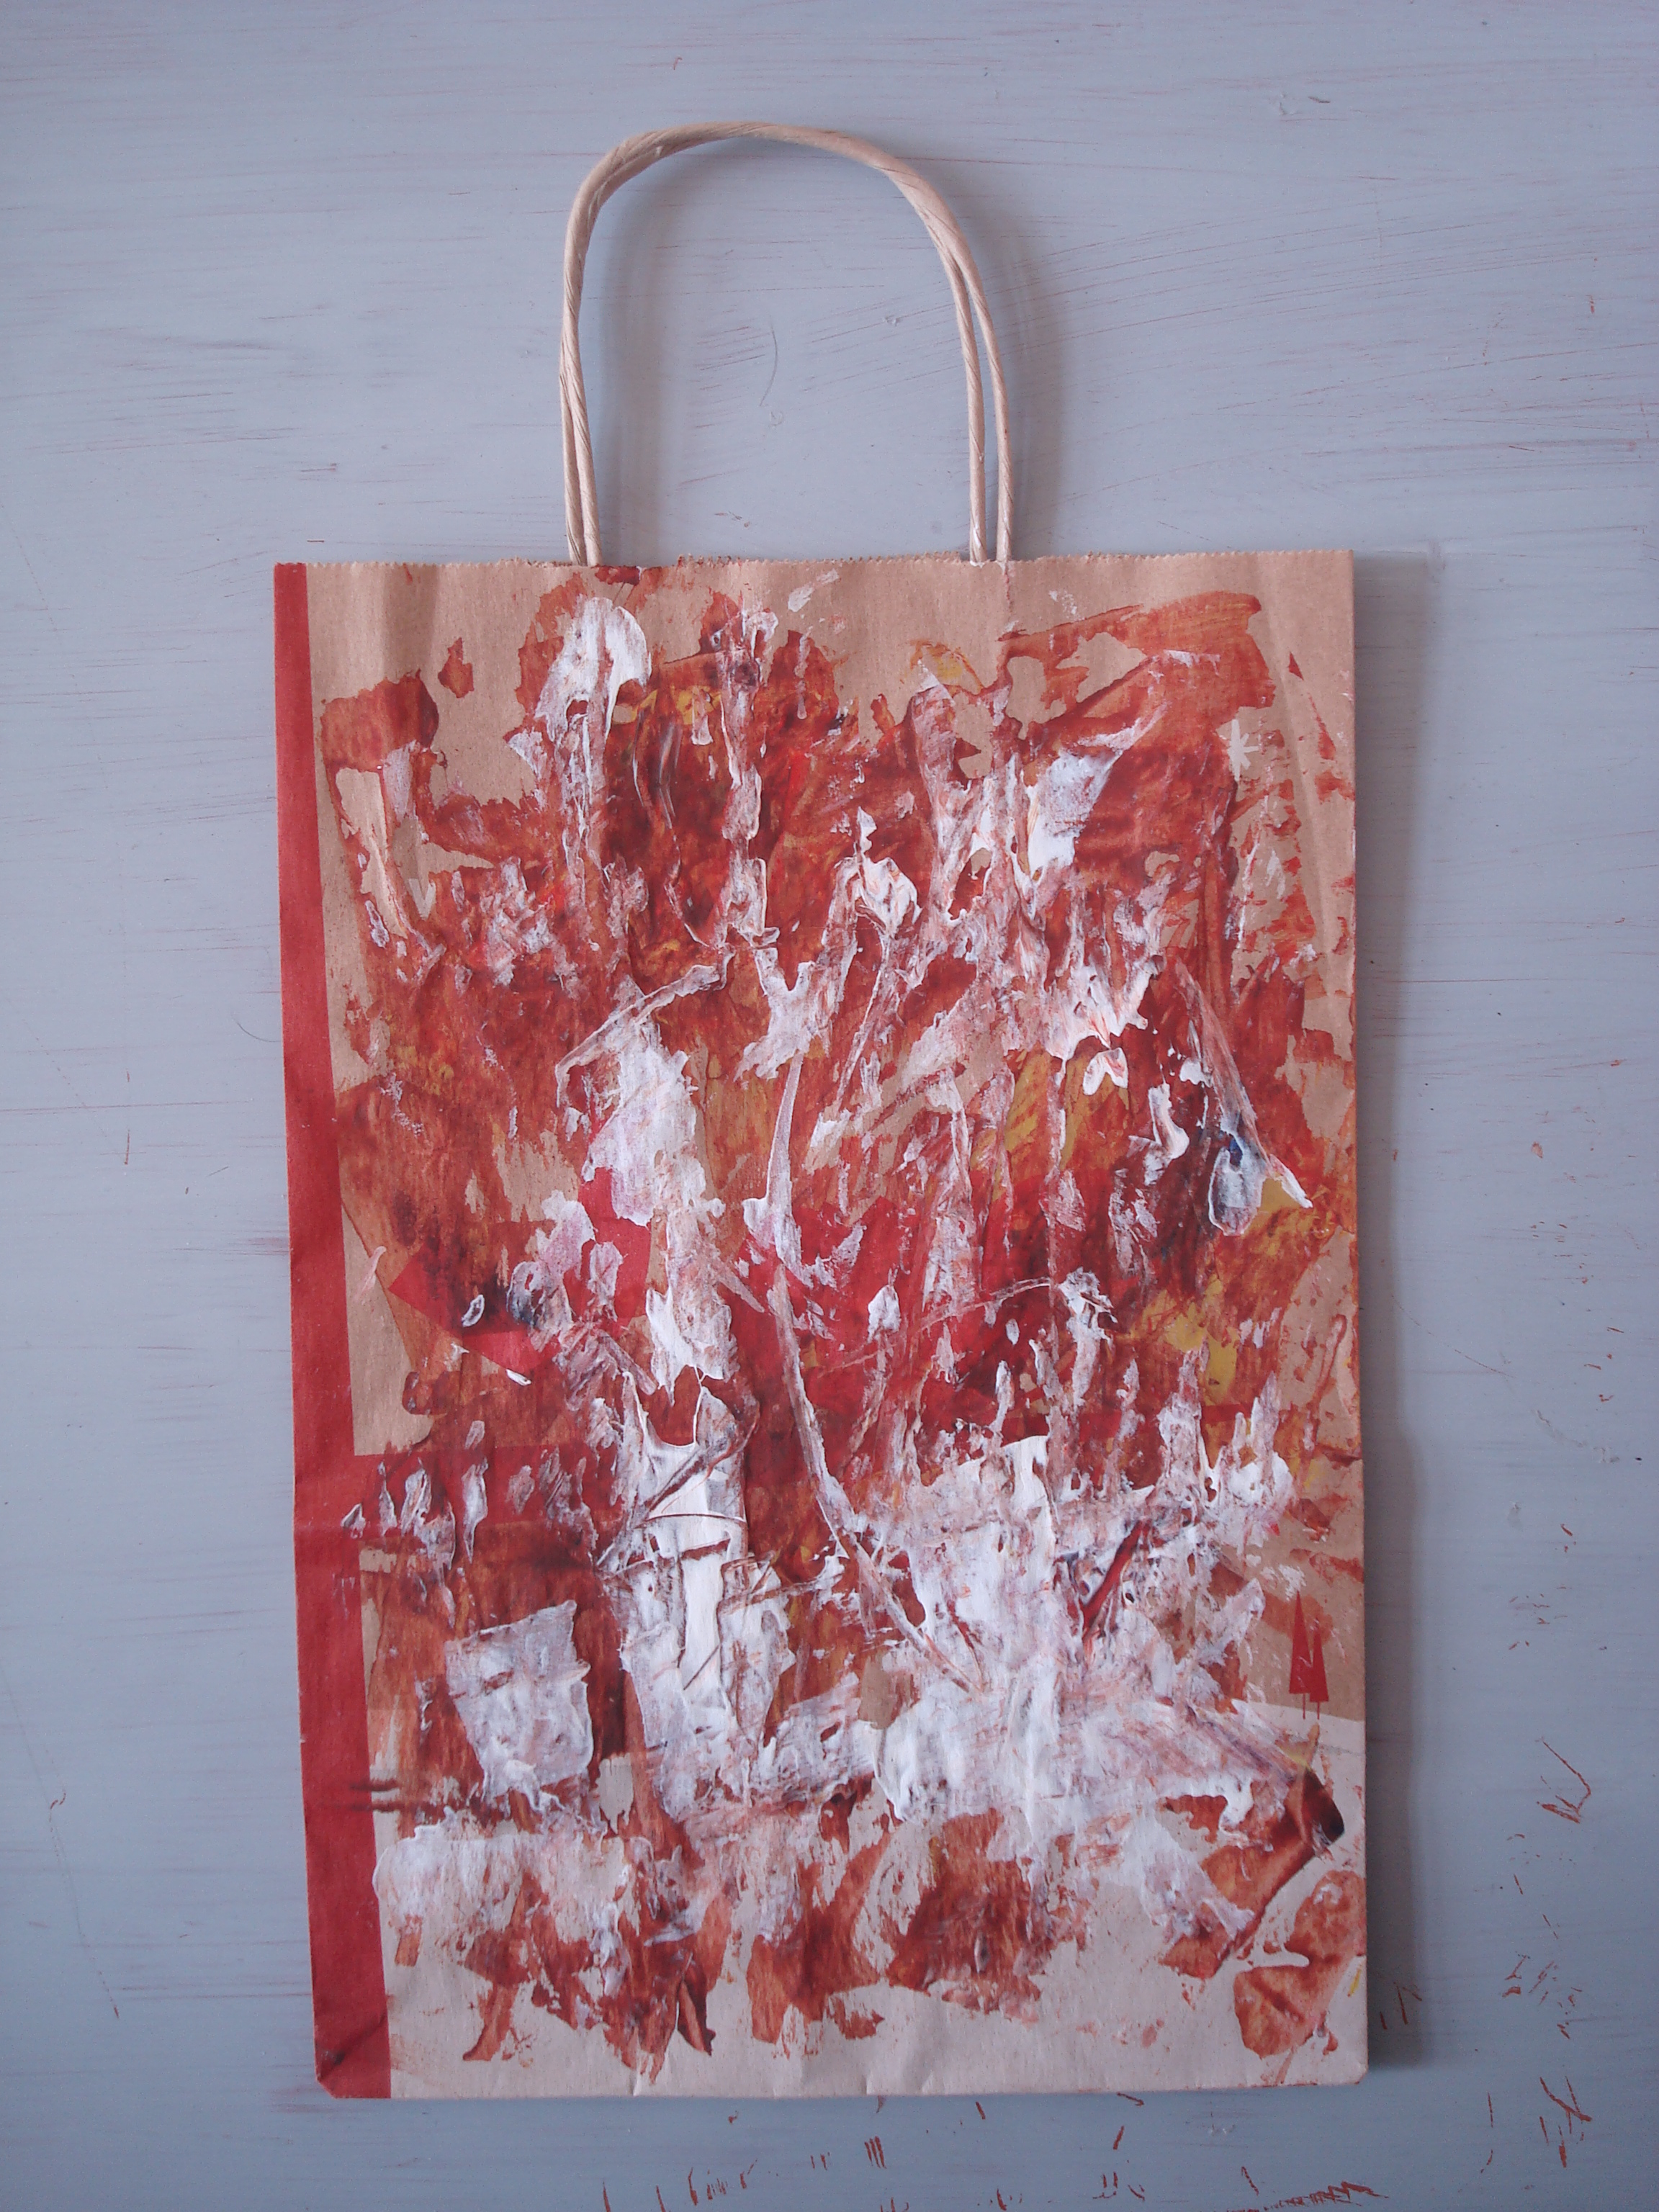
\includegraphics[width=\textwidth]{project_graphics/early_works1.jpg}
    \end{subfigure}
    \begin{subfigure}[b]{0.30\textwidth}
        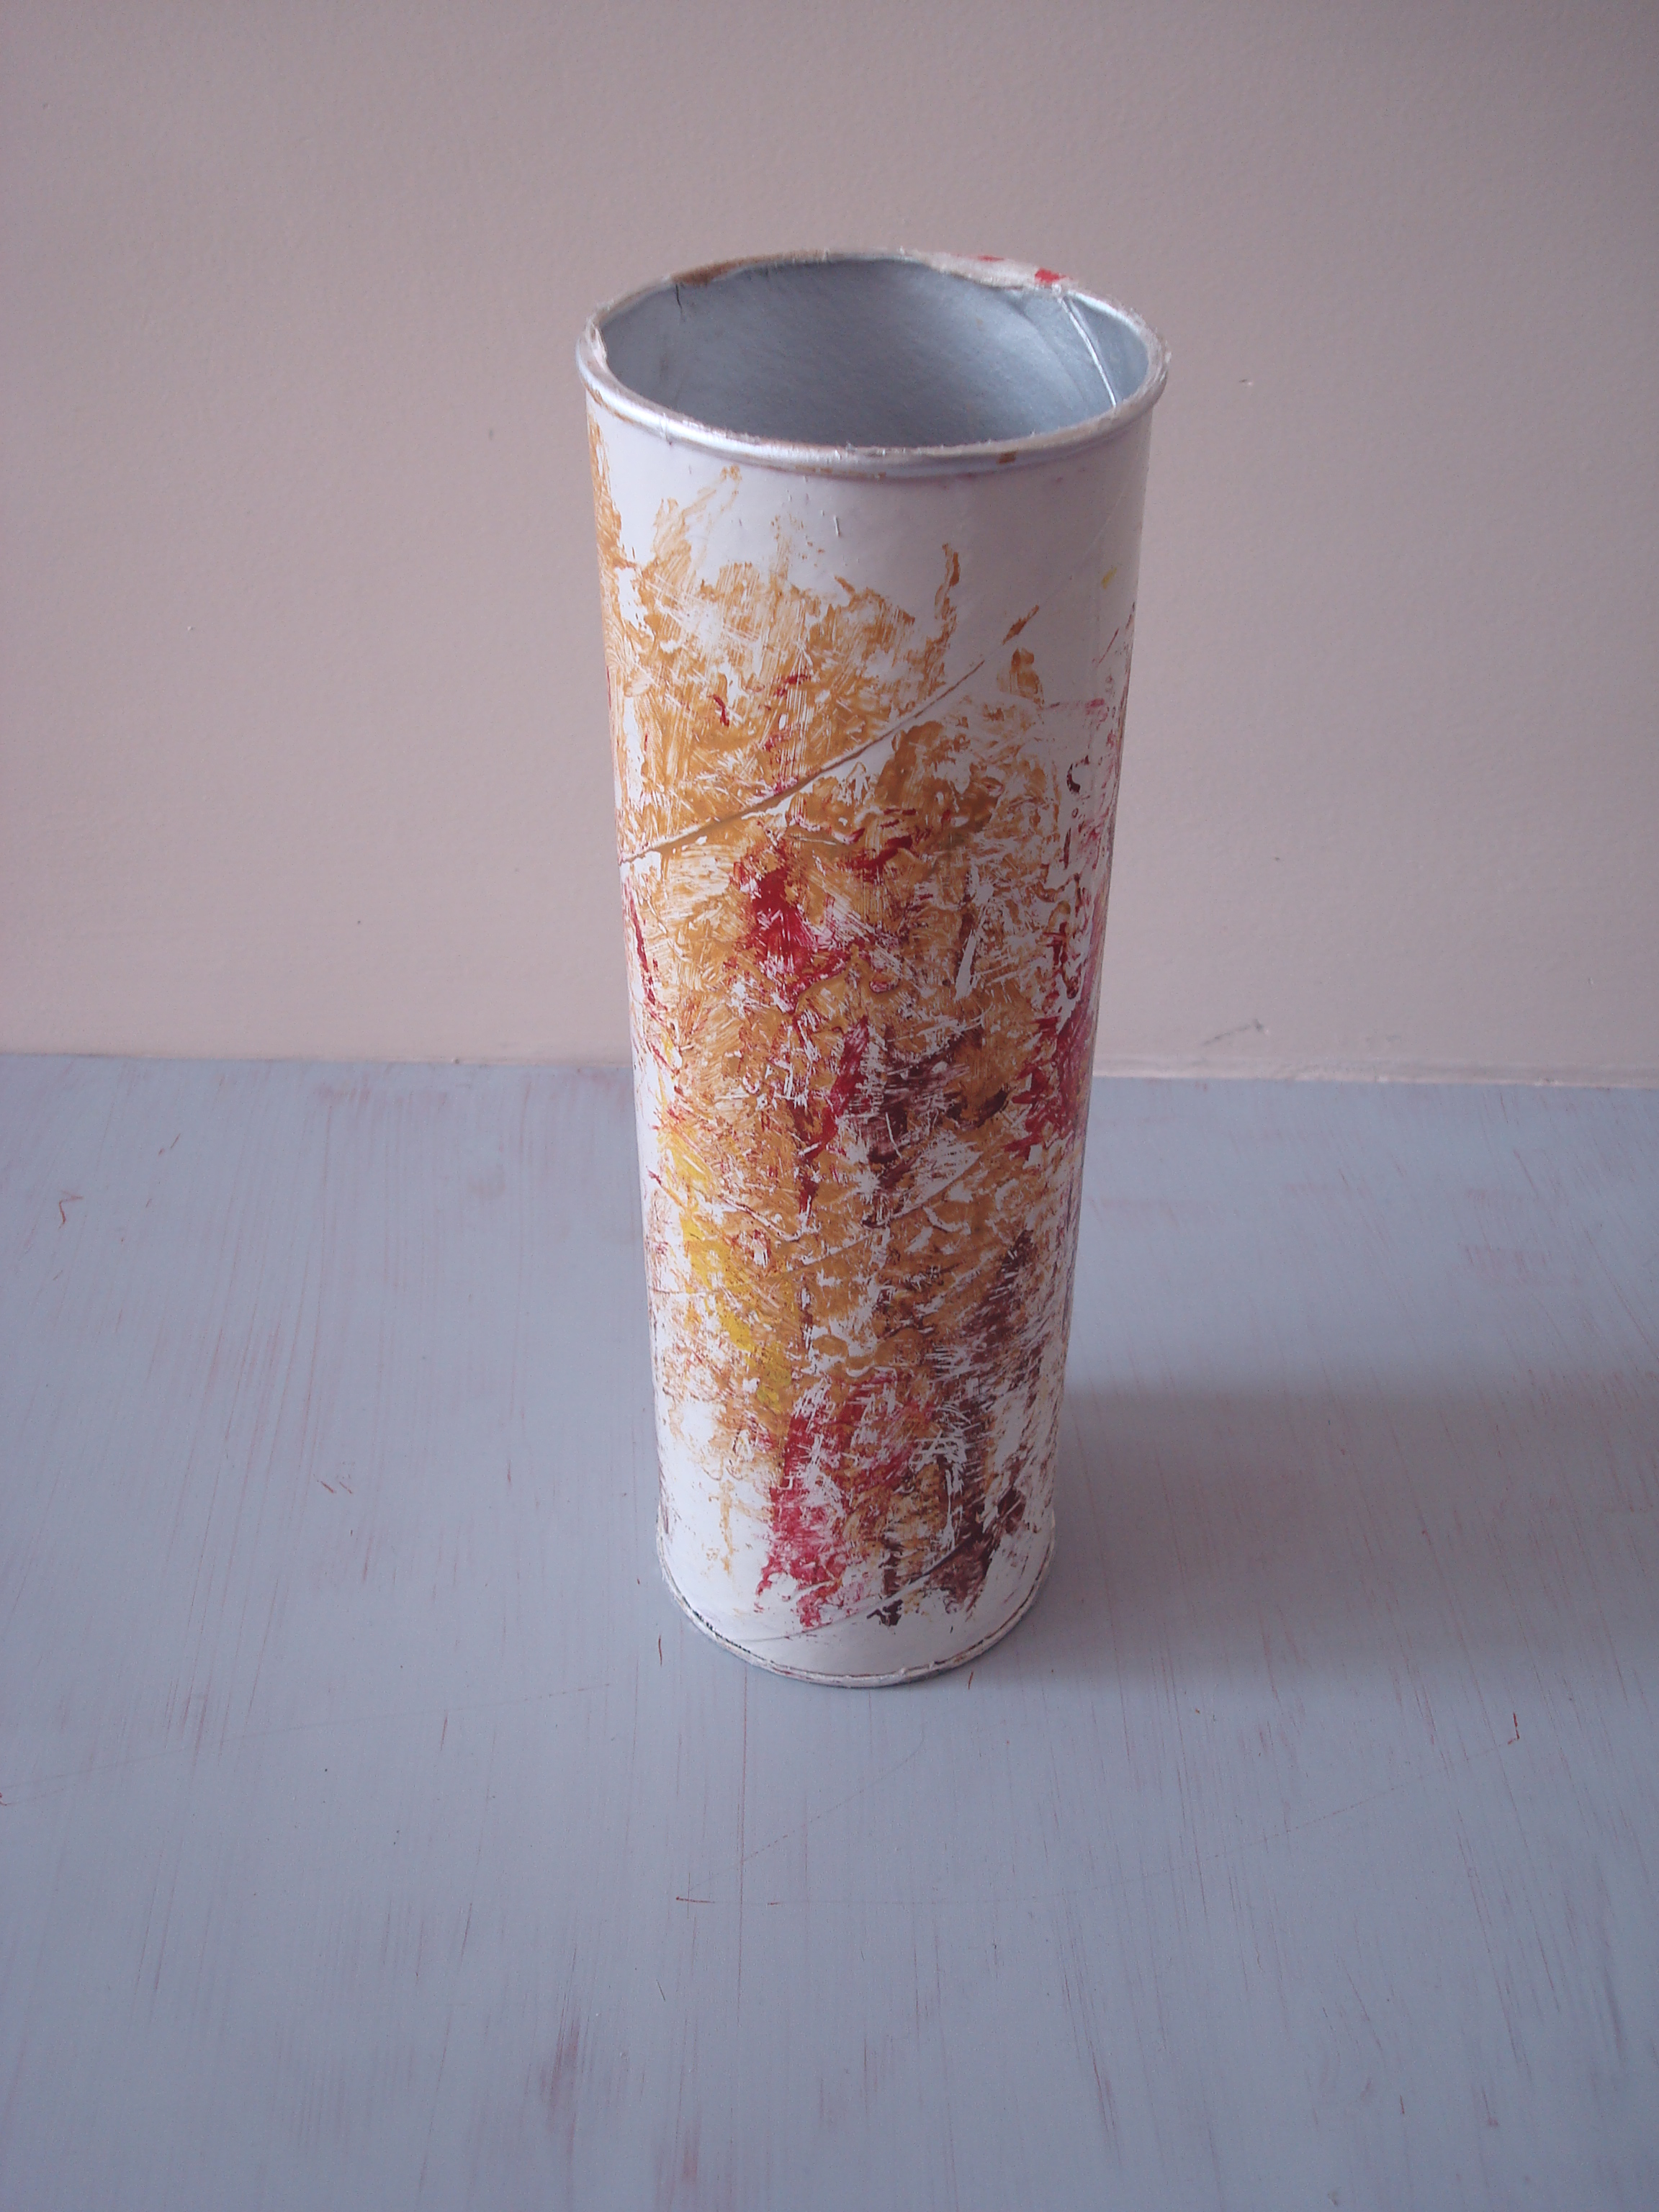
\includegraphics[width=\textwidth]{project_graphics/early_works2.jpg}
    \end{subfigure}
    \begin{subfigure}[b]{0.30\textwidth}
        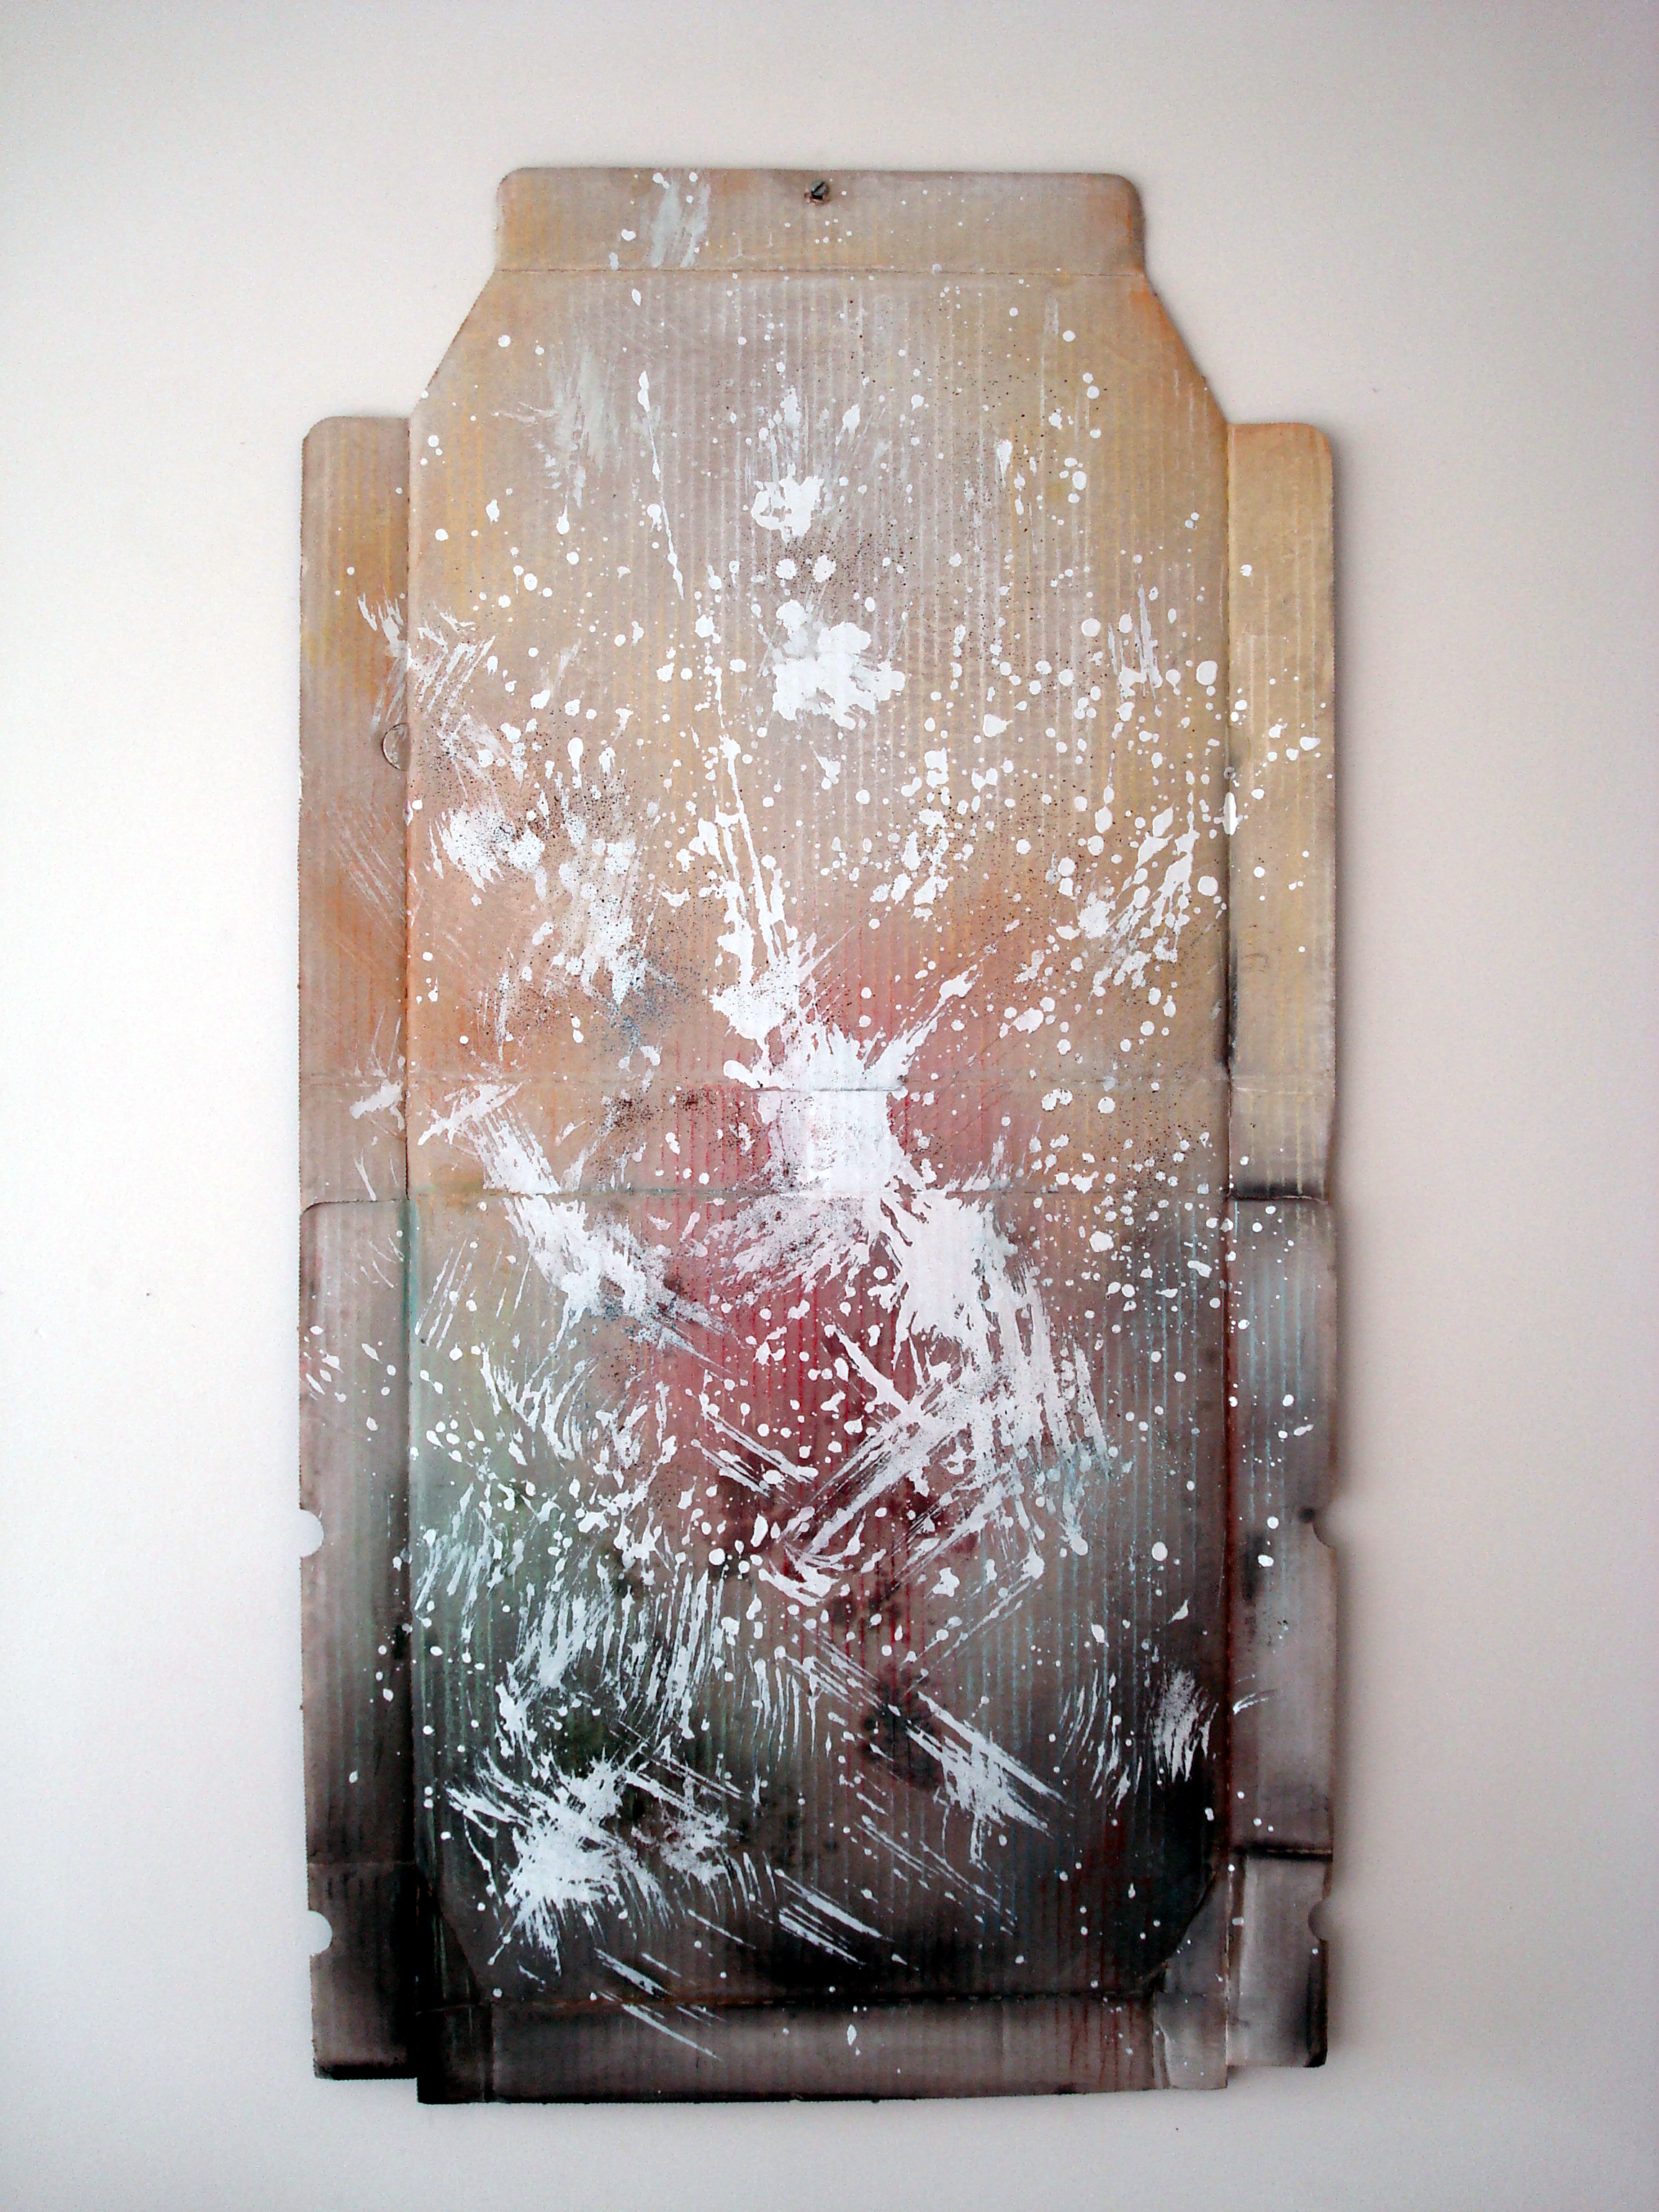
\includegraphics[width=\textwidth]{project_graphics/early_works3.jpg}
    \end{subfigure}
    \caption{Examples of early works}
    \label{fig:EarlyWorks}
\end{figure}

After turning discarded materials to different uses I began to collect them more eagerly. At the same time I also gave what I did to my friends as a birthday gift. I was experimenting with the material and at some point with the help of my mother I made my first notebook covered by Starbucks package. Papers inside of it are blank mimeograph paper which different than white paper. Particularly purpose is to move away from white paper because I feel uncomfortable when using it. It looks to me very bright. Therefore mimeograph paper is better for me. At that time it was a great victory for me. I started to carry it and use it every possible place. I show them to people and some of them supported to me giving their discard. One of them is my supervisor. He started to collect packages for me. After turning his packages to notebooks, he suggested me to go deeper in this subject and make my thesis project from them. Thereafter what I need is more discarded material.

% But covering things are not new actually, when we are primary school again, we cover our books and notebooks. My mother, she is also a teacher, still covers her books things whatever at hand. (I have remembered that we are covering our notebooks at school. Sometimes we also cover the books.)

% bir yandan free olması experiment yapmak için ideal olması.

%\textbf{What do I think about trash?} I need to clarify my approach to the trash, wasting and discarding. First point is that I am very uncomfortable to the action of discarding thing. I always think that by discarding this think I am missing something rather than getting rid of something. Sometimes because of the significant amount of residue from consumption from daily activities I became overwhelmed and to move on I need to leave behind them and move on. However almost it is never ending loop. (I believe that sometimes we need to break the loops to realize different meanings. To think outside the box, we need to behave outside of common habits. As I mentioned the discarding things are some of the loops that we are rare to behave like other way.) \textbf{What am I discarding?} To get rid of my load and move on. But for what? and also ought to be like that? (throw away them to same bin. (Some of people do not care too much bin and throw them whenever it is possible.)) Even if I discard some stuff I think that I am ignoring its potential and losing it. At that times I become very sad and feel very comfortable. I must have find to another place for it more suitable than a waste bin. At least I can give them someone else who can use it for own purposes. Do I really luxury of discard?

%Significance of thinking outside of the box (about trash) is actually breaking the loops. You have to look at differently from common perception. \textbf{Break the rules, break the loops} to realize the alternative. \comment{Even if the market gives many alternatives of commodities, why do people still seek the alternative? Is not is enough? What type of gap that industrial products can not fill the gaps. Neden tüm insanlara hitap etmiyor?}

%[Making exploration.] One of the encouraging factor is to work on trash is to find (or explore) something different from someone else's discard. Because it is ignored by discarding and therefore undiscovered. Wait us to be discovered. and possiblely (as picasso mentioned) discovered again and again. \comment{Different people from different culture bring new interperation, but it is exist all of things.}

%It contains evraka moments.

%[Motivation.] I can not throw them away. When I throw them I became sad for them. I have to find something useful for it. (Failure of imagination, failure of making meaning) Even if I can not find it, I can pass it to another person who can make use of it for own purposes. There is a lot of effort to produce objects and it seems that all this efforts are wasted. What I mention is not related about ultimate productivity. It is more close to being thoughtful, and taking responsibility of tools, items and objects that we are using. Rather than throwing out, creating a way that all are have chance to live together is much more close to my perception.

% Önceki chapterlarda insanların kişisel olarak objelerde neler buldukları önemliydi. Ben de burada kendiminkini anlatacağım. Benim için yeni bir şeyler üretmek için birer kaynak.





% NEW PART [collecting] 
Collecting discarded objects has carried out through the efforts of mine and people around me. Lars Eighner's instructions helped me a lot when collecting objects. He writes that 
\begin{singlespace}
\begin{quote}
Eating safely from the Dumpsters involves three principles, using the senses and common sense to evaluate the condition of the found materials, knowing the Dumpsters of a given area and checking them regularly, and seeking always to answer the question \singlequotes{Why was this discarded?} \citep[as cited in][6]{strasser1999waste}.
\end{quote}
\end{singlespace}
I applied these instructions to my case and I checked some points regularly and seek the reason of why was it discarded. Details will be given later for each objects. 

% Bozulduğu için mi yoksa şekli standartlara uygun düşmediği için mi atılmış agnes varda da gösterildiği gibi.

% [Mode of search] looking for waste bins. asking for people. realizing during the daily life. for example bank splits.
% ofis, varuna, bilkent labı gibi mekanlar aslında önemli. benim malzemelerin büyük kısmını bulduğum yerler. iş bankası mesela. found photos.

Moreover there are other rules that define the frame of collecting act. Paper or package must be trash or will be trashed. For this project anything must not intentionally bought to use as trash. In other words first rule is to consume less and generate less trash. Lots of trash is accessible. Aim is to reach them.

%[owner of disard]
\quotes{The question of who owns these discards is not trivial} \cite{zimring2012encyclopedia}. This question makes me uncomfortable because of feeling that stealing that someone elses' objects. Particularly I felt it when collecting leaved out papers from Bilkent Computer Laboratory.

% http://newsroom.ucla.edu/stories/studying-trash-as-art-249200
%Trash is also regarded differently, depending on where you live. Last year, an undergrad in Zubiaurre’s honors collegium seminar went to a poor neighborhood and scavenged through people’s trash; no one cared, Zubiaurre said. But when the same student went to Beverly Hills to go through trash, the police were nearly called. “Who decides what is public and what is private? How come trash becomes highly private in a rich neighborhood, but truly disposable in a poor neighborhood?” Zubiaurre said.

% bırakıldığını nasıl anlıyordum vs.

%[people]
% Bu kısmın daha güzel anlatılması gerekli.
% TODO ref.
As mentioned previously many people contributed to the project by collecting. Whenever i meet my friends I ask them to save their discard. The importance of collaboration with them can be understood the term "citizen science" which is \quotes{defined as scientific research performed in part or in whole by volunteers who are not professional scientists} \citep{robson2012using}. I need to note that this is not a scientific project but the notion belongs there. The value of it lies in the collective intelligence of the contributors. In the scope of this thesis the term can be interpreted as people bring their own creativity and interpretation to the project by collecting the items that they reach and select. When the number of contributors are increased the diversity of the collected material will be increased and this will echoed in the notebooks. 

It can be viewed as a co-authored work. Because many people helped me to collect the papers and also many people leave their trail to the paper and also they bring meaning to the them. After production of papers I also want them to continue as co-authored process. In other words many people will be part of this project. As people see different things on objects and bring them to me. the variety of things is increased in time. Because people sad me that \quotes{I thought that you can use it. Do you collect also these?}. After that time I want to continue as so.

% They provide me the materials to transform it. They select the items and find them. They bring their approach and selection. They are part of the selection of the materials. They started to engage with the work. People bring the material also wonder the result of it.

% taxi drivers is wonder what will happen? they can not understand the idea here. not only collectors wonder but also people see me in action wonder the reason of it.

The purpose is here not only to transform objects but also change the perceptions of trash. Asking people to collect things and inform them started to shift in peoples mind. For instance 

Collected items reflect my and contributors' consumption practices. People as mentioned previously consumption patterns can be tracked from their leftover. From logos of companies onto the packages reveal people's choices and give clues about their social status.

% TODO What type of activities generates waste.
% Beyond social status it reveals activities that generate such a waste.
It can be also extracted that most of the trashed papers are thrown away from feeding activity. On the other hand vastness of some types of disposables reveal the dark side of the some enterprises such as Starbucks and Burger King. Few people thought that after seeing the project I only collected Starbucks packets. There is no such a limitation but as a result of habitat the number of them suppress the others.

%[disposable paper, packaging]
Collected items are mainly disposables ones. Most of them are paper or contains paper pulp. The word paper comes from papyrus, the plant that was first used for writing in ancient Egypt long before the making of paper in China. It is fundamental medium for writing, reading, education, communication, information storage and many others. Its role in the development of human civilization can not be neglected. (Paper in several forms is consumed on a daily basis \cite{trafford2012paper}.) Wide range of use from packing to newspaper makes it indispensable product for people. On the other hand for artist it offers great diversity in order to make compositions as can be seen in the works of collage. Further it is easy to find and collect them. Even if it is thrown out, still appropriate for painting and writing.

% TODO: Free ve accessible olması experiment yapmak için önemli bir yere getiriyor onu.

% [Production, Recycling] \paraphrase{All types and qualities of paper share the same basic method of manufacture, including newspaper paper, print paper, and carton used for boxes. Paper made exclusively from wood is called virgin paper, while paper produced out of used paper that is re-pulped is called recycled paper. Recycling paper can greatly diminish demand for virgin fiber from wood. However, there will always be a demand for virgin paper because, although paper is thought of as a renewable resource, it cannot be recycled indefinitely. It can only be recycled four to six times, as the fibers get shorter and weaker each time. In addition, some virgin pulp must be introduced into the process each time to maintain the strength and quality of the fiber, so no matter how much is recycled, paper will always need some virgin fiber.}

Since paper is both biodegradable and a renewable resource, it is preferred by some of corporations for their products to show their respect to the nature. The motivation why they use can be seen their notes printed on the papers (Figure \ref{fig:NoteOnPackage}).

\begin{figure}[h!]
  \centering
  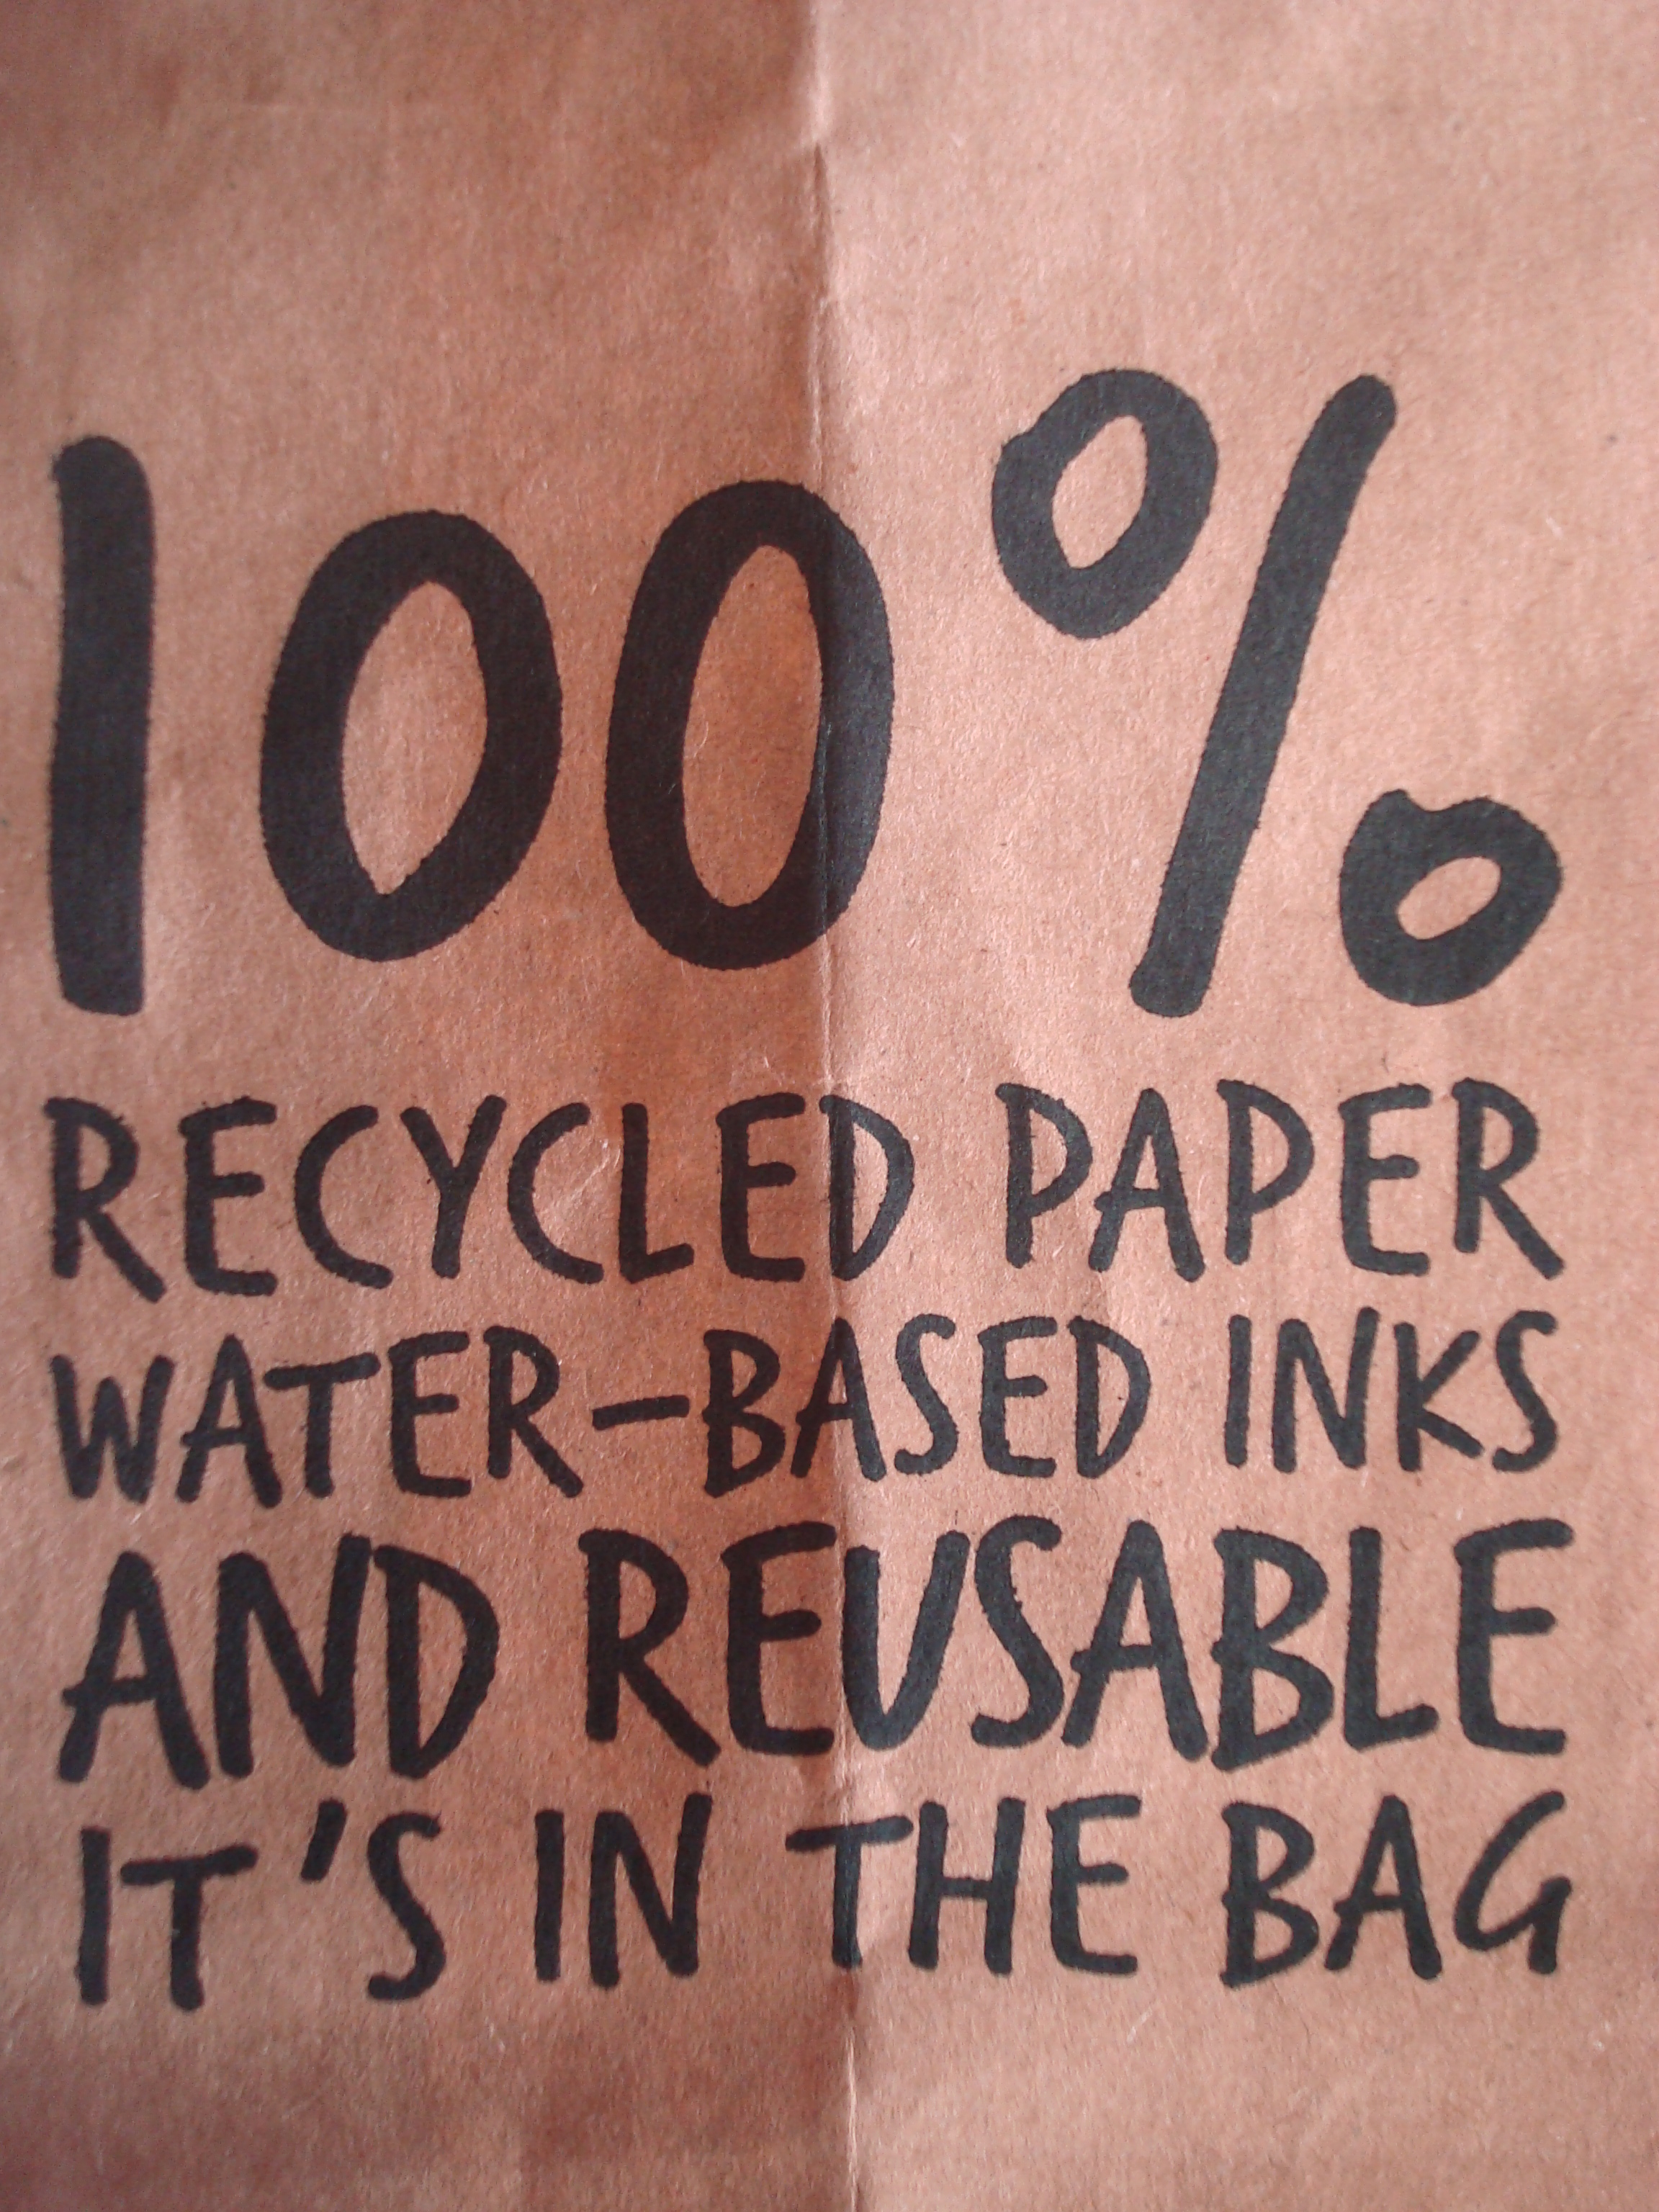
\includegraphics[height=6cm]{project_graphics/recycled_note.jpg}
  \caption{Recycling notice on the package}
  \label{fig:NoteOnPackage}
\end{figure}

% meaning of paper for me.
% TODO buraya bir şey eklenecek.
%Seeing papers on the waste bin is a disappointment for me. As stated by the artist Aaron Kramer \quotes{Trash is the failure of imagination} \cite{meyer2007turning}.

% [Why do I collect trash?] Herkes neye ihtiyacı var ise onu toplar. Ben neden niçin topluyorum? Toplama sebepleri? Dönüştürme sebepleri. Neden sadece toplamakla yetinmiyorum. yani toplamak ile ayrıldığı noktalar nelerdir. Ben bir mana mı arıyorum? Yoksa kaybetmekten mi korkuyorum? Yeni kompozisyonlar oluşturmak istiyorum. Farklı karşımlar elde etmek istiyorum. Bir tür şaşırtmak durumu... Beklenmeyeni yapmak... En olmadık malzeme çöple çalışmak bu yüzden önemli benim için.

Collected items are stored in my room. All of they are varies. Most of them are not belong to me. Here the detailed information of the collected materials are listed.

\begin{figure}[h!]
  \centering
  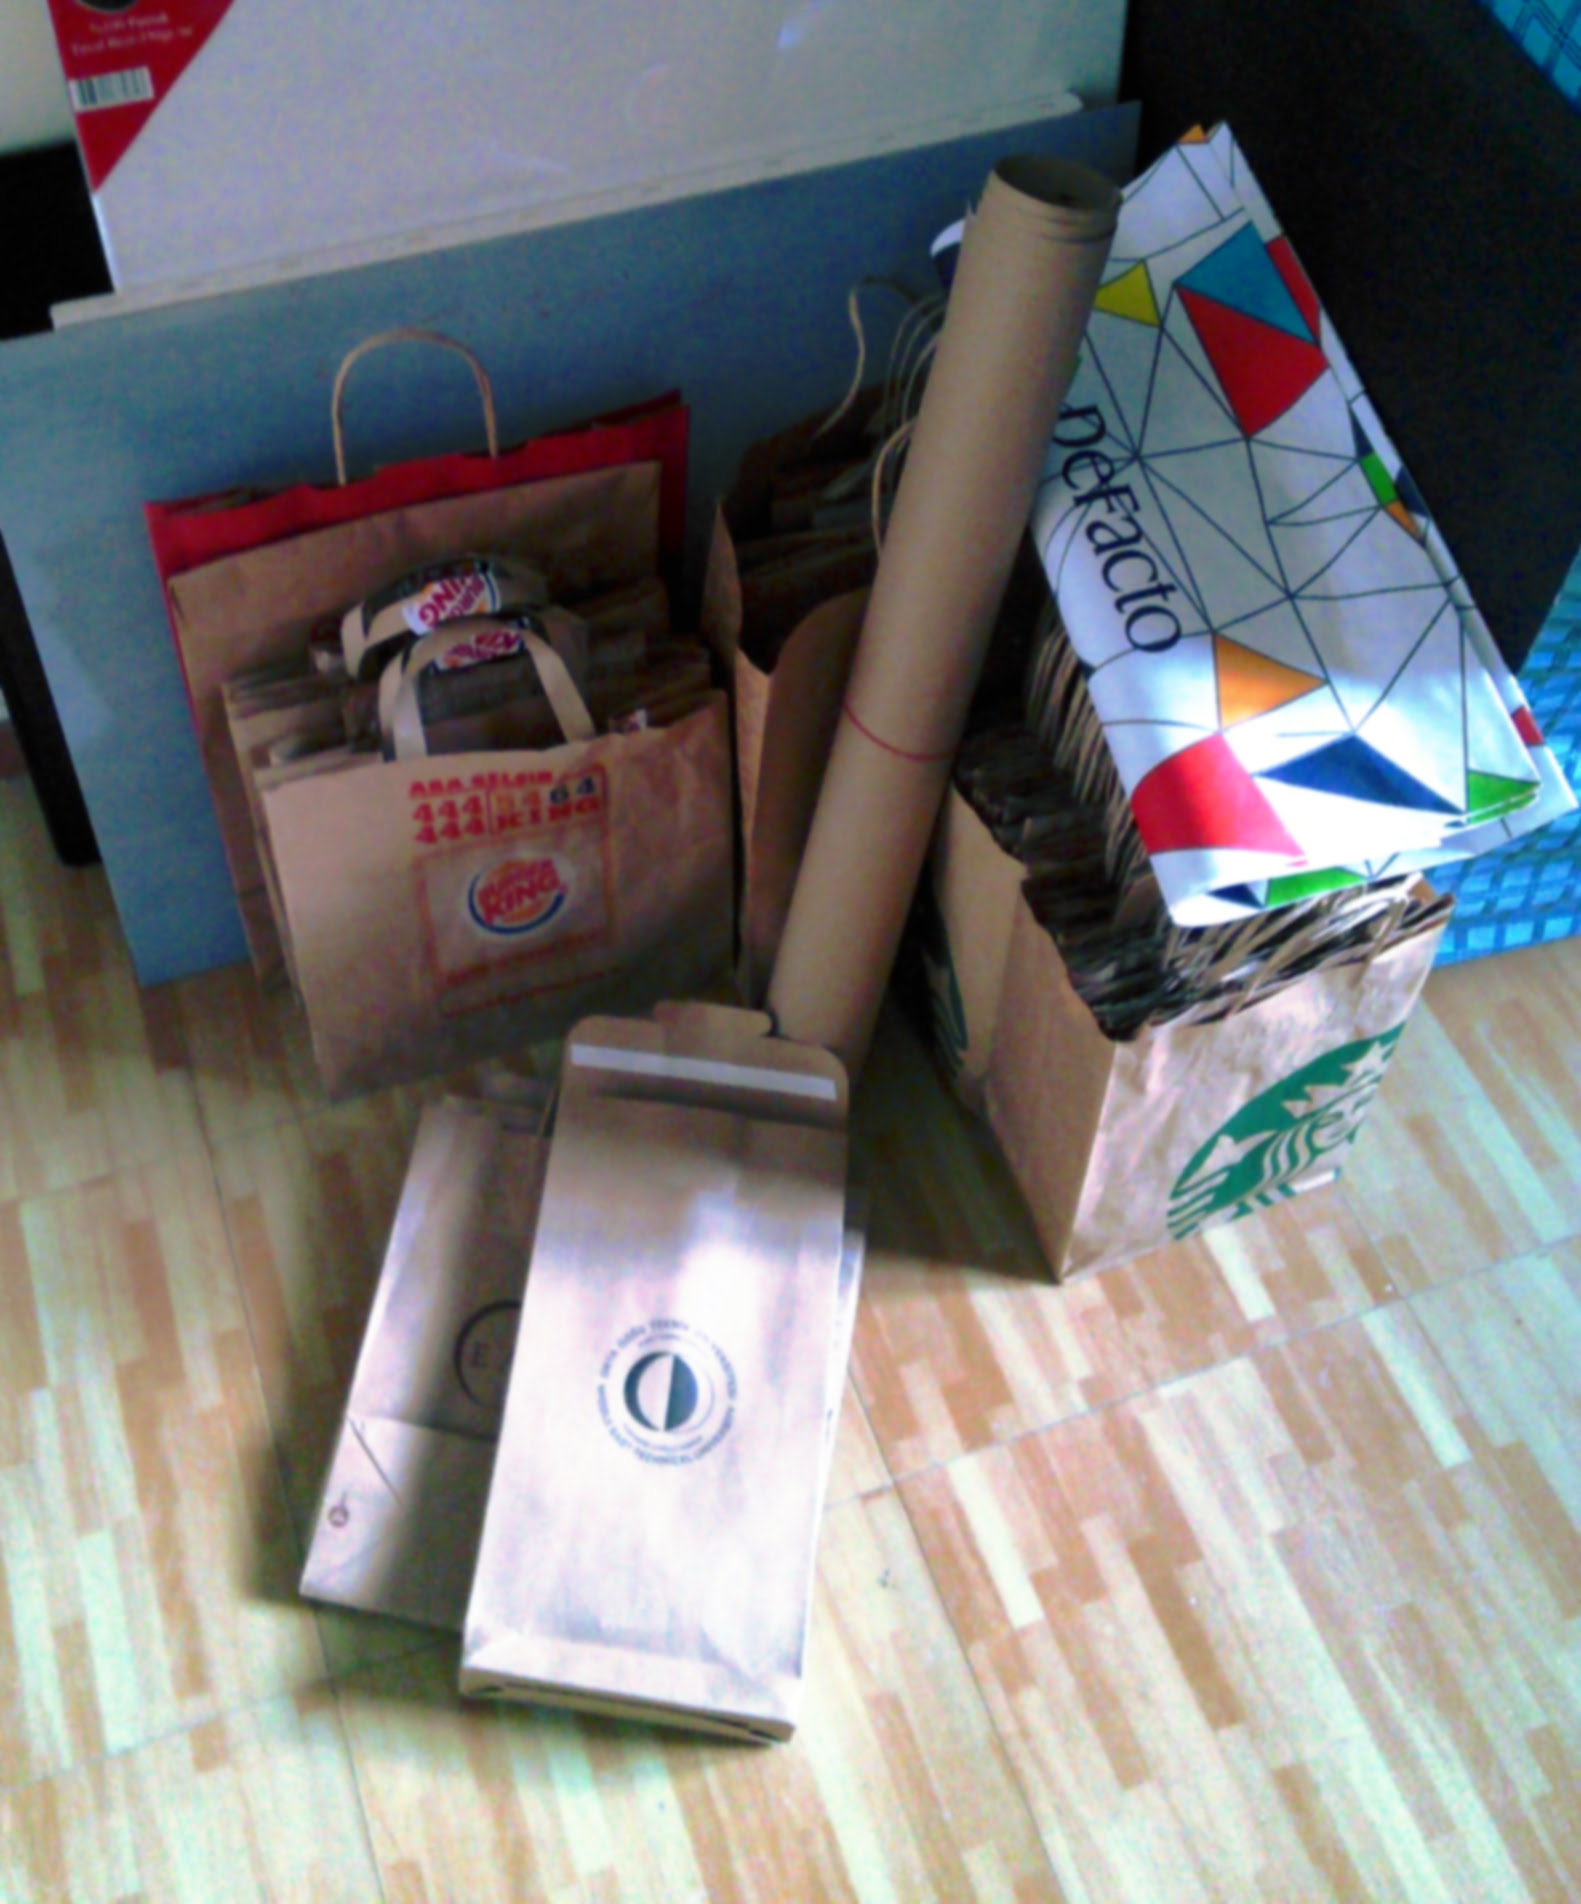
\includegraphics[height=10cm]{project_graphics/collected_all_together.jpg}
  \caption{Collected materials}
  \label{fig:CollectedAllTogether}
\end{figure}

\textbf{Burger King packages} are collected from the office where I work. At launch time, some of the colleagues order the meal from Burger King which is a global chain of hamburger fast food restaurants. Meals are delivered to the office with paper packages. The package of the meal is collected and used as a cover of notebooks. 

%Also one paper package is used for French fries which is greasy and paper is very good to absorb greasy. Some people think that it is disgusting because of greasy onto it. But immediately I replied them just not you eat that greasy fires so what is wrong with it. At that time what Susan Strassed said comes my mind. (it fits here)

Why people throw them away varies. Through my experience I can give one anecdote that I encounter frequently. When I collect the papers under the dishes or food packages, people often think that it is disgusting and called them as dirty. However, it is very strange that the fat on the paper was previously what they are eating.

\textbf{Starbucks packages} are collected from my supervisor, office and my friend. Especially my supervisor and friend saved and collected them from their friends. They are used as a cover of notebooks. There are different types of packets from this category. for some of them are build from recycled (precisely downcycled) paper, and the others packages for coffee beans. they are airtight and waterproof packages very solid and strong. and well graphic design with different color and illustration.

\textbf{Modshifters papers} that are covered on table and at the end of the day they are cut out and throw away. I go this place many times and every time questioned what they are doing to the papers. One of my visit we stay there at a late time and catch the garson collecting the old papers and preparing tables to the next customer or day. I ask him to give me and he kindly accepted. From this paper I covered [x] notebooks. All of them contains track of people who sit down there. I do not know them and I am not sure that the paper that they are sit down turned to such a thing.

\textbf{Varuna Gezgin}, is a cafe. papers of old menus. They are waited to be discarded. 

\textbf{Graduation banner} Because it is cut out from very big and long banner (which is carried at graduation ceremony at METU, 2011). Every piece was a part of bigger banner. At that time there are serious debates about freedom on the internet. Most of the website are banned from the decision to the courts and they were not accessible. (Access to this banner is blocked by a court decision.) In Middle East Technical University there is a tradition that in graduation ceremony people walk through in the stadium and greet to the tribunes. With this event they carry some banners to express their feelings and criticize some realities in the country. This one of them. It is carried by students (new grads of Computer Engineering) The slogan decided by among the students and before the ceremony I printed out the slogan to carried out as many people as it can and easy to readable from the people who seat at the tribunes. After the ceremony I could not throw away this banner. I do not know what to do it, it is very big actually to store but I could not. I think that I will figure out later. Maybe I can use it as a draft paper. But is it worth to cut out this all long banner etc. Also to strengthen the banner and to prevent to tear while carried by the many people we are tape it from its boundaries. In other words some of the areas can not appropriate for writing. When I decided to this topic I remembered to this banner. It is stands in a corner in a dusty way. Now it is time use it. It waited very log time and it is time to revive again. Currently In turkey the problem of banning web-sites continues. Event it can said that people do not surprises when a website is blocked by the courts. It can be turn be a paper that people can freely express their ideas and feeling onto the it. Cut out them to the smaller pieces and make them as notebooks. They are part of puzzle. for the smaller parts what is written on them can not easily understandable. To realize what is the message is you have to bring together all of them again. But It is not possible, therefore website is a very good solution for them. All pages have unique patterns. Remaining parts of letter and tape. It provides unique layout for writing and I strongly think that all the notebooks after used have strong visual impact.

\begin{figure}[h!]
  \centering
  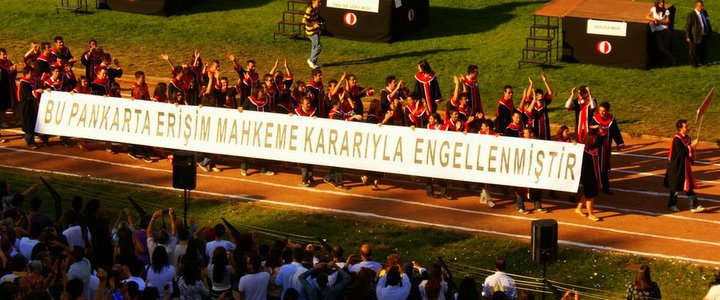
\includegraphics[width=1\textwidth]{project_graphics/banner1.jpg}
  \caption{Banner}
  \label{fig:Banner_1}
\end{figure}

\textbf{Tea bags} are collected from my friend. Their a couple of consumption of tea and their covers.

\textbf{Order slips} are collected from bank office my discovery at bank. opening all perceptions. After that I really convinced that I am really looking for trash everywhere every time.
% [Everywhere, everytime, Life practice.] En başta bahsettiğim everywhere, everytime aslında collecting ile çok yakından ilgili. Bu toplama işlemi normal hayatın içine sızıyor(infiltrate the life). iş bankası örneğinde anlatılabilir. bir de art gallery found object örneği verilebilir.

\textbf{Elginden gelen kağıtlar}

\textbf{Bilkent kağıtları} % bu kısım found photos ile ilişkilendirilebilir.

\textbf{Others} collected items are not limited with these by the remanings are little to open a new category.

%as it can be seen here there are various types of paper and most of them some memories for me.???





% NEW PART [transforming]
%[experiments with paper.]

% TODO sadece defter yapmakla uğraşmadım bşka şeyler de denedim.

% [Artistic tactics] Here I followed some tactics to accomplish my purposes. Easy to carry while traveling. Small notebooks. Placing them to their routes.

% bi de ben bunu insanlara vermek istiyordum o yüzden defter iyi bir şey. ve bu benim aslında bir taktiğim arkadaş. defter insanın yanında taşıdığı kullandığı bir şey. sadece galeri de olmayan başka alanlara da sızan bir şey olması önemli. 

% sadece belli bir yerde geösterile bir şey olmayıp yayılan, insanlarla birlikte hareket eden bir şey olmasını istiyorum.

At one side while paper is being collected, on the other side I started to make experiments with the material. I questioned what else can be made with these collected materials and tried to cover (wrap out) objects and plants in the public. However these do not give the result what I want. People cannot interact with these and possibly they will turn to trash again. For that reason the first approach which is making notebooks are more appropriate to accomplish the purpose.

\begin{figure}
    \centering
    \begin{subfigure}[b]{0.47\textwidth}
        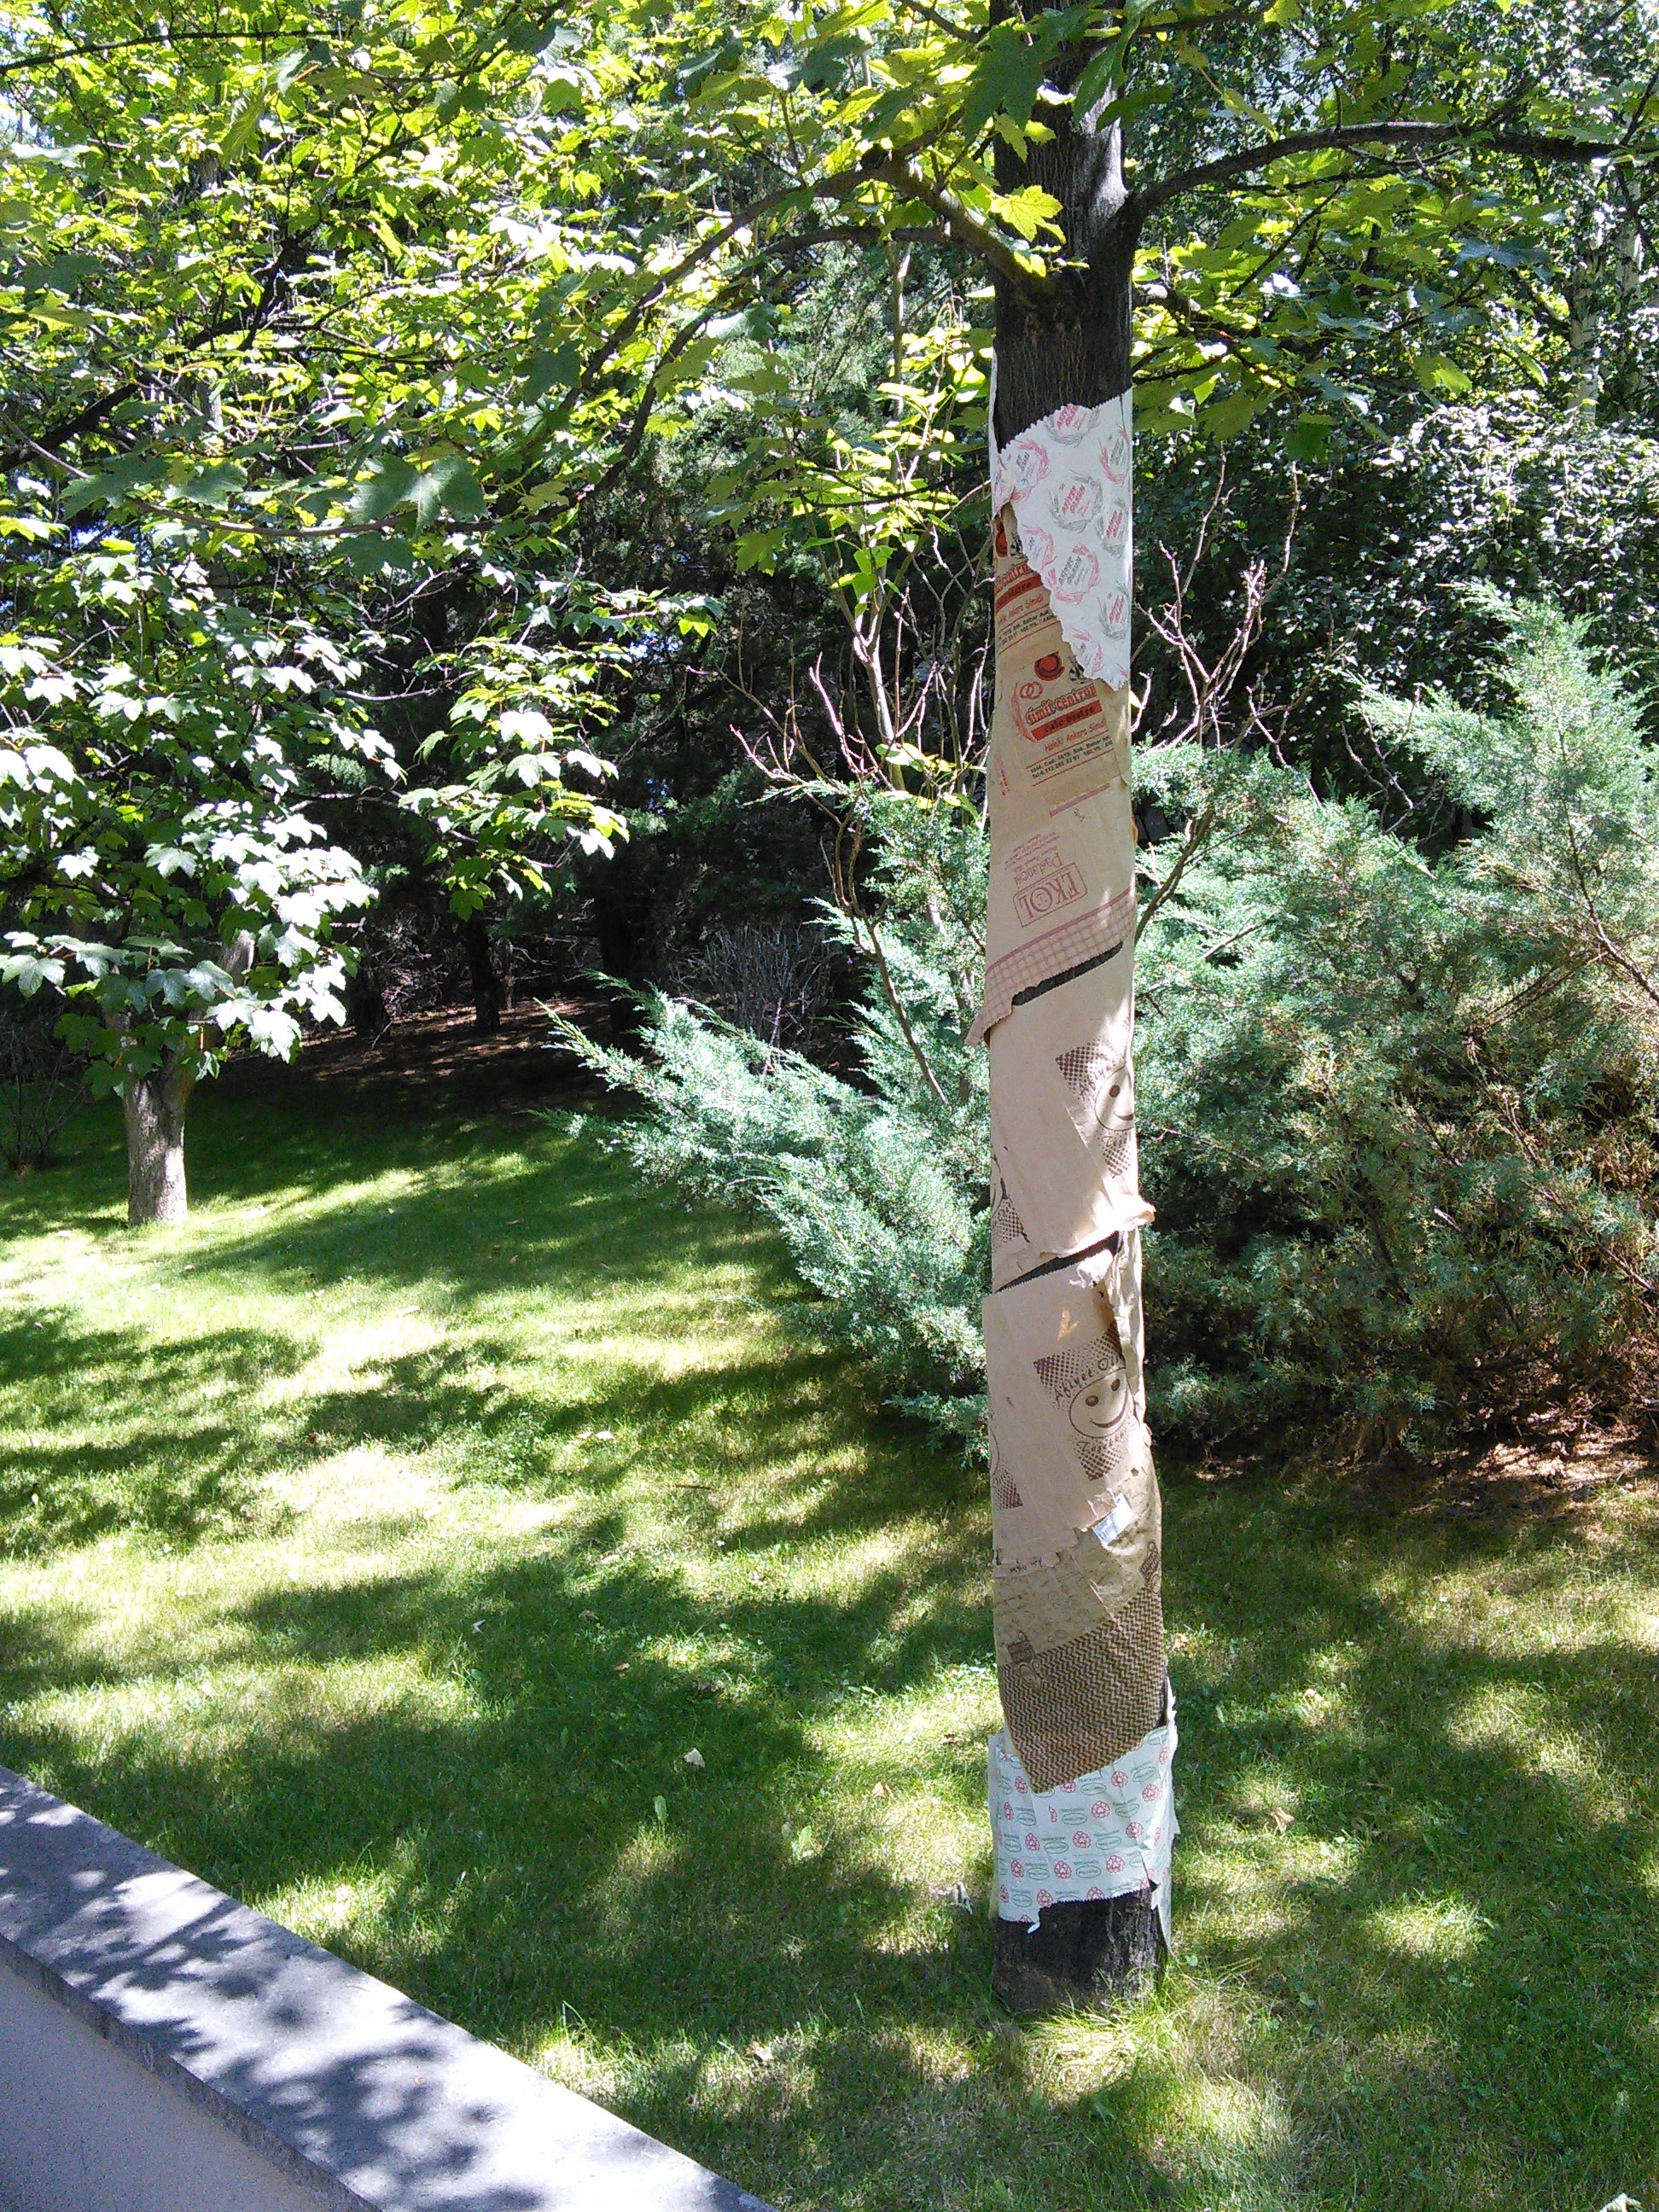
\includegraphics[width=\textwidth]{project_graphics/tree_experiment1.jpg}
    \end{subfigure}
    \begin{subfigure}[b]{0.47\textwidth}
        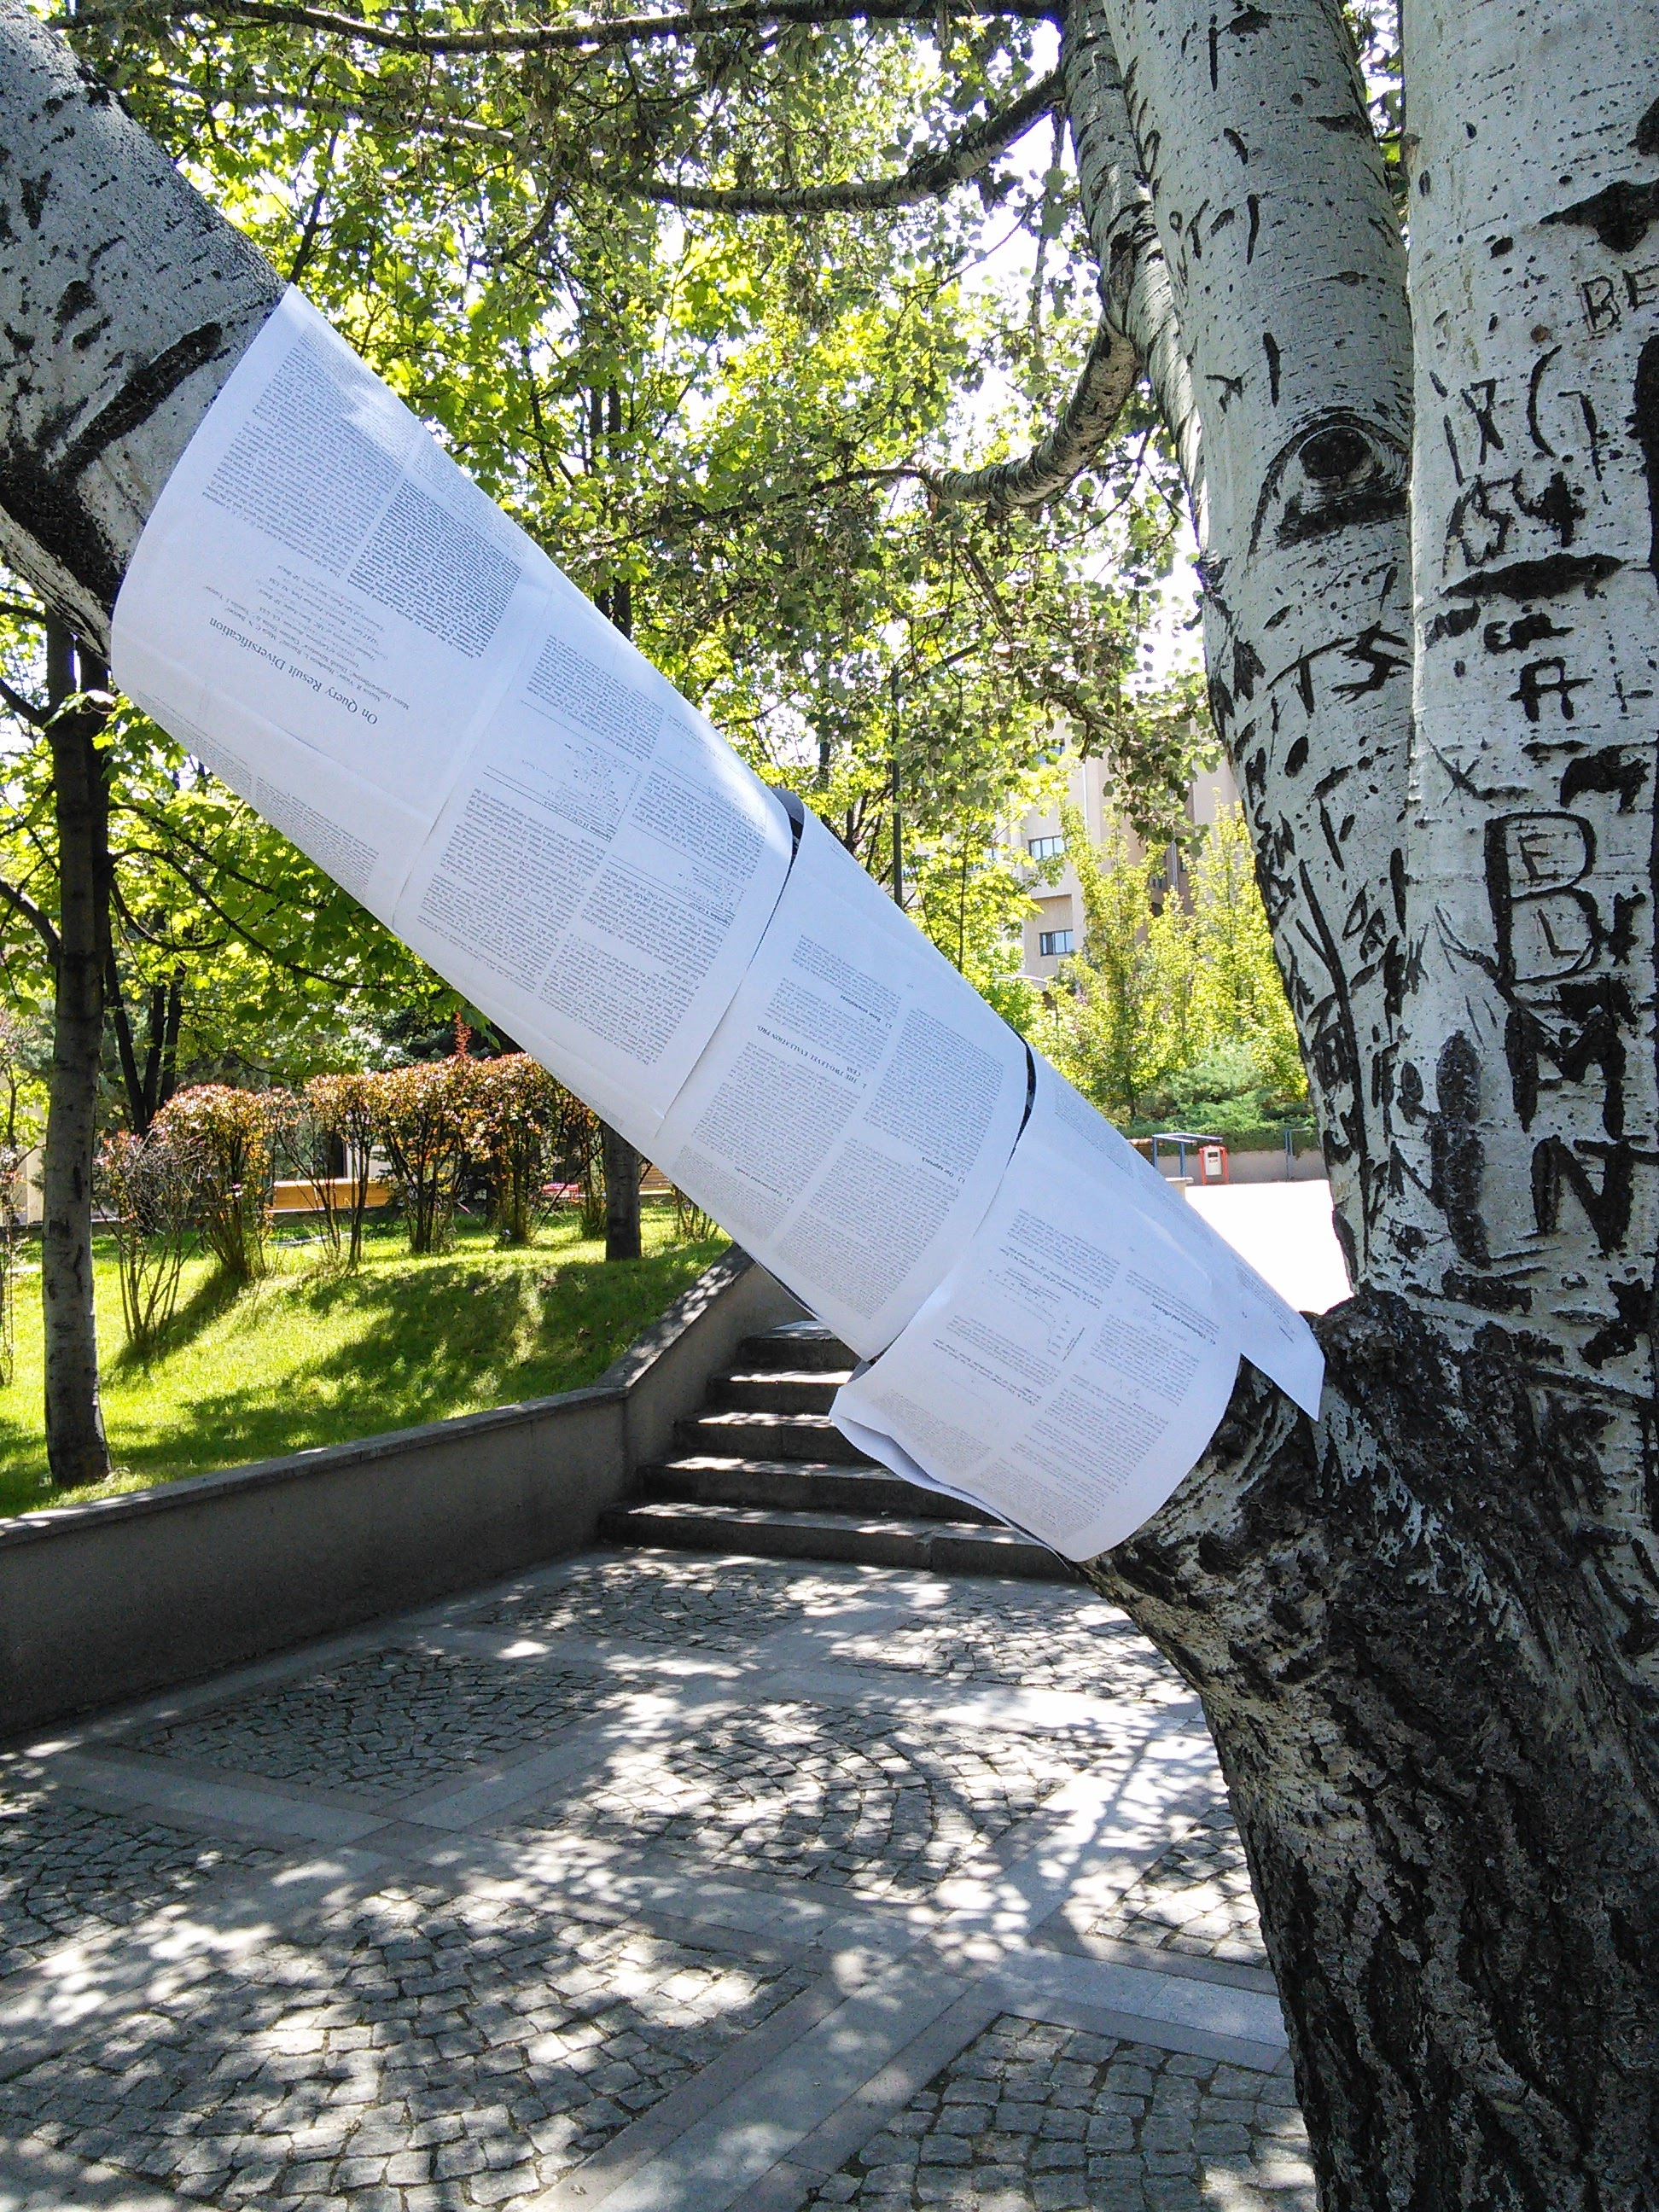
\includegraphics[width=\textwidth]{project_graphics/tree_experiment2.jpg}
    \end{subfigure}
    \caption{Experiments with collected paper}
    \label{fig:ExperimentWithPaper}
\end{figure}

% [notebooks]
Papers that are mostly blank(empty) are used inside of the notebooks for writing. Others that are solid and colorful are used as a cover for notebooks. Mixing (juxtaposing) materials is main method in the production process. I combine different papers and packages. I try to generate every possible combination. The purpose is to create as many alternatives as I can because trash is ignored and people do not give it new alternatives. Therefore these notebooks provide many alternatives to show that otherwise is possible. 

Technically papers combined together by sewing and gluing. I learned sewing techniques from my mother and the gluing part is trivial. For this project I need to produce dozens of notebooks. However through time I started to produce them more rapid by improving my technique. One of the struggles that I faced is to punch holes with needle. At this process I cracked a needle. Later I discovered that with the help of pushpin punching the holes becomes more easy. After punching holes I just followed the holes with needle. I used nylon yarn which is solid and thin. Being thin is important it must fit into the opened holes. After sewing them I fixed the yarn with hole by gluing to make it more solid.

% TODO starbucks defterlerinin hep yapıştırılmış olmasını da eklemek gerekli.

% TODO muhakkak tekrar kontrol etmek gerekli.
Size of the paper used inside of the notebooks are mostly equals to the size of an A4 sheet. Usage of papers differs among the notebooks. Especially for the papers taken from Varuna Gezgin written part is folded inward by hiding it. However for the ones collected from Bilkent Computer Laboratory written side of it leaved open. Their content comes from various students whose departments are also various. In other words offers great diversity and they are mixed to allow different interpretations. Further it provides what students from other departments works on. % What other students work on.

% TODO Dimensions of notebooks. most of them half of A4 or quarte of it. böyle bir fotoğraf eklenmeli. farklı boyutlarda farklı şekillerde ve renklerde.

% TODO sabahleyin bir fotoğrafını çek bunların.

% TODO defterin yakından fotoğrafları

% TODO kullandığım malzemelerin listesi olabilir. fotoğraf çok fazla olur.

Moreover I have reviewed other notebook projects. Notable ones are The Sketchbook Project and myDetour from Moleskine. In these projects anyone who bought the notebooks from them can participate and send their notebooks filled with illustrations and paintings. These projects can be seen as crowd-sourced library. Further the pages of the notebooks are available at online. After checking sketches in these notebooks, the diversity of them surprised me a lot. It forced me think that the transformation process is not limited with the production of notebooks from trash. After notebooks are given to the people, their transformation will continue. Therefore I think the process of transformation is a continuous act.
% amaç çeşitliliği arttırmak olduğu için 

% TODO siteye nasıl karar verdin la?




% [showing]
% [Exhibiting experiments] main question id how to give them to people?
After producing notebooks the most important point is to present and reach to people. Starting point is to stack the notebooks onto the each other, and there are other ideas like putting them inside a waste bin to re-do the action of throwing away. After ward somehow they should understand that these notebooks can be taken. I set up makets and tried some installations of them.

\begin{figure}
    \centering
    \begin{subfigure}[b]{0.3\textwidth}
        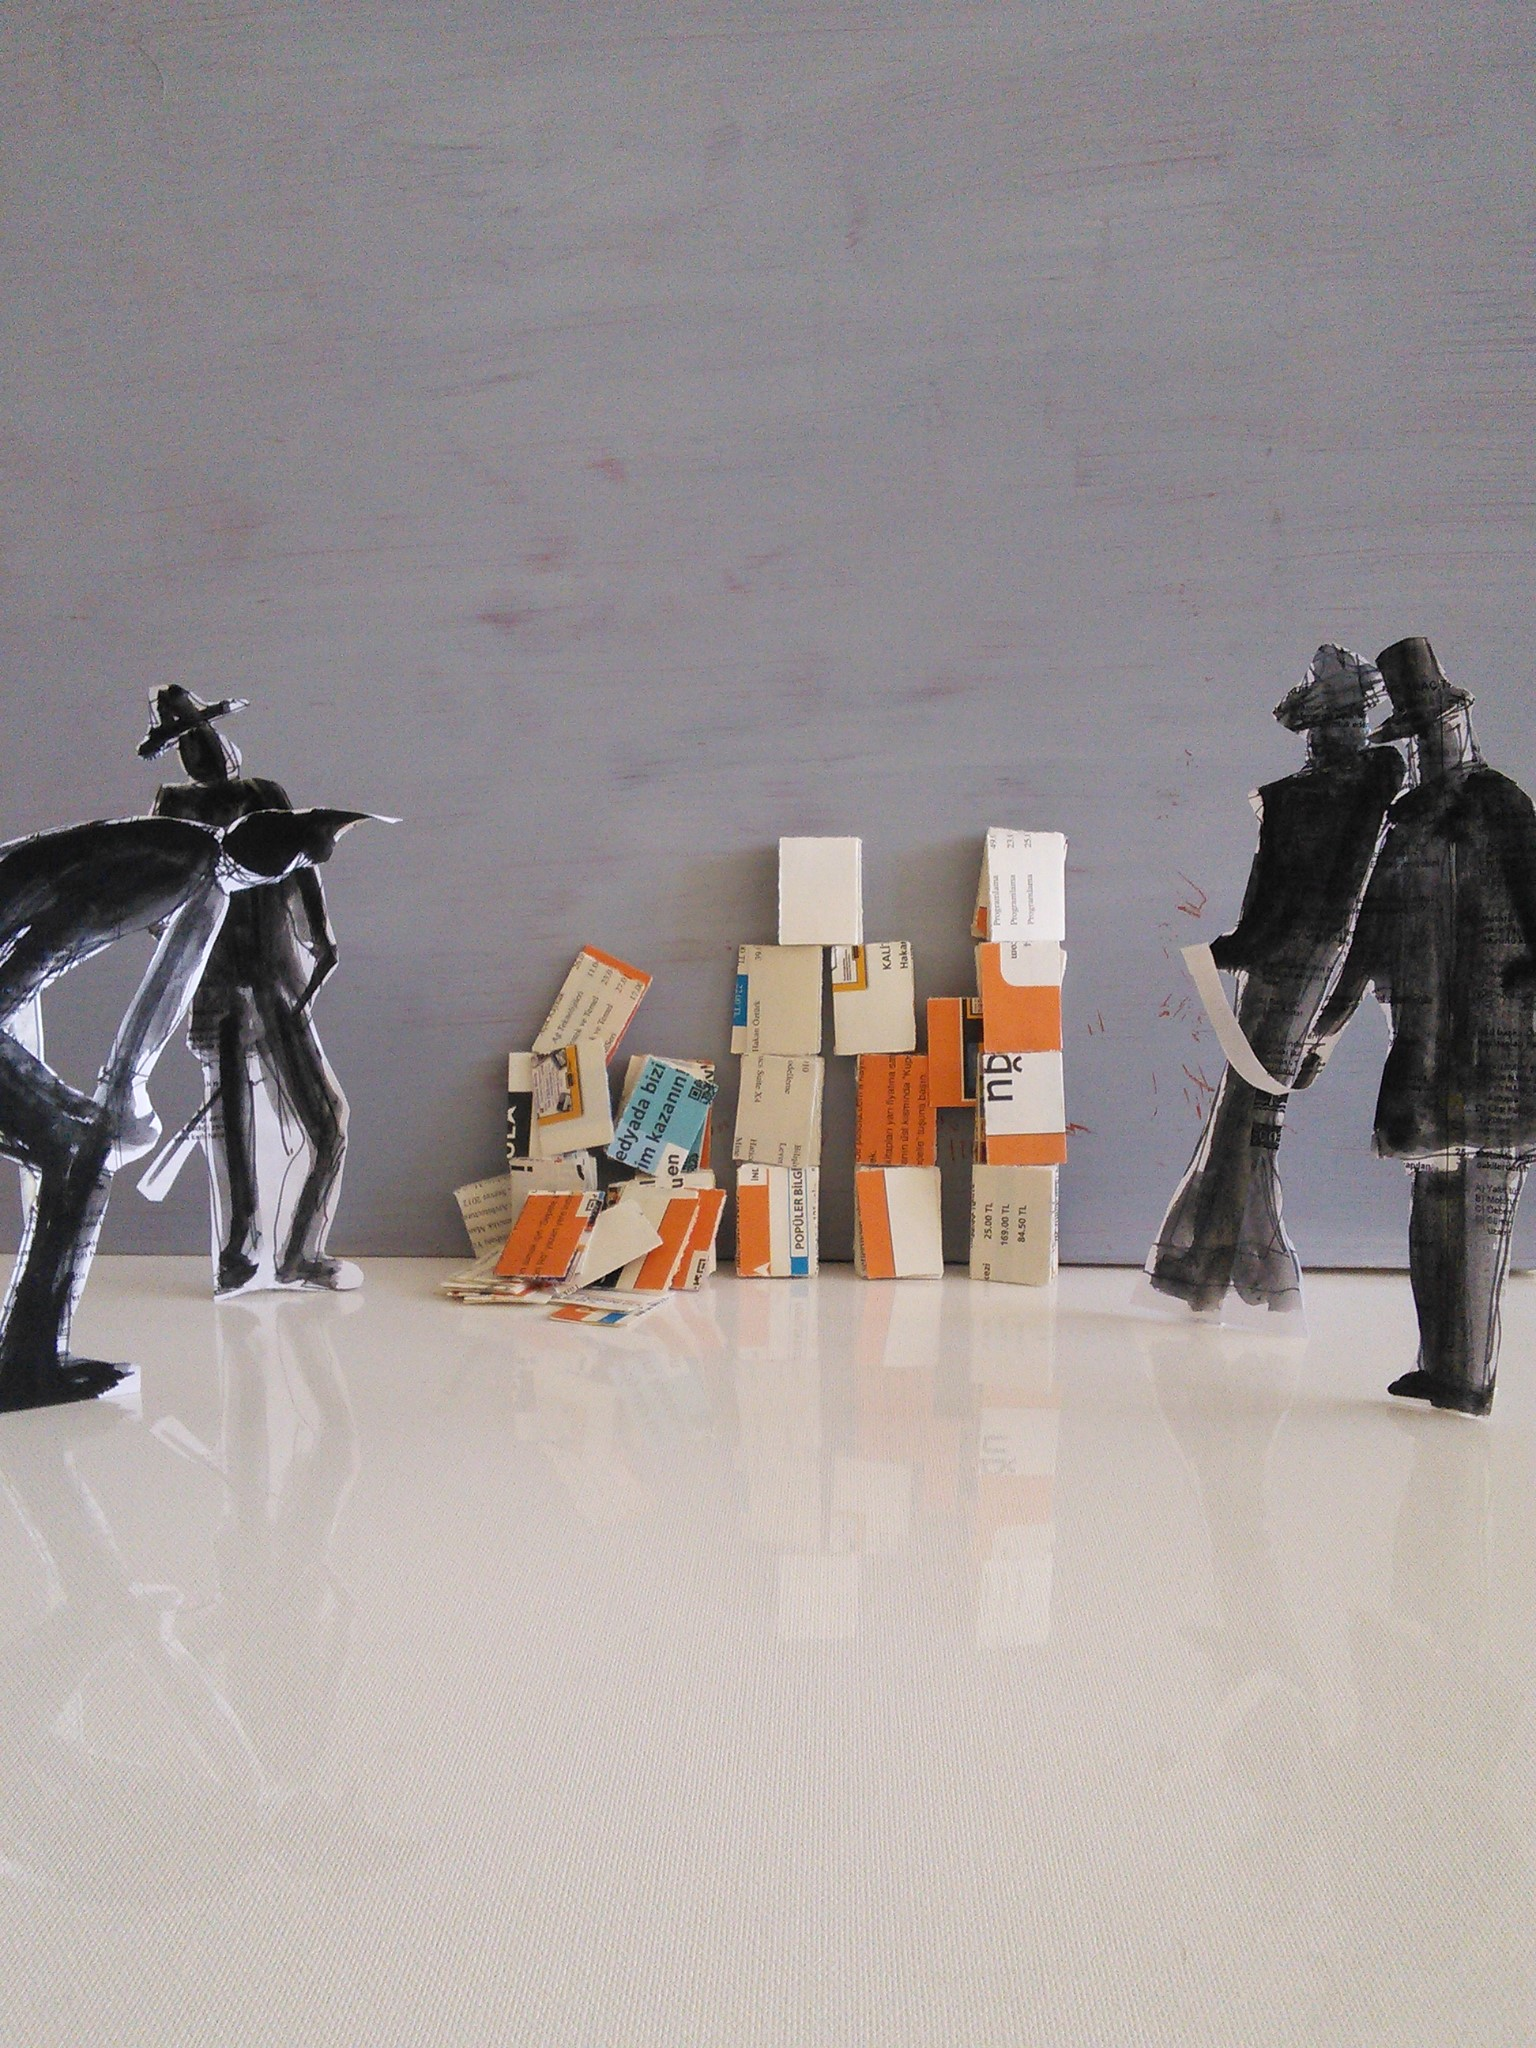
\includegraphics[width=\textwidth]{project_graphics/exhibition1.jpg}
        %\caption{Sax}
        \label{fig:exhibition1}
    \end{subfigure}
    \begin{subfigure}[b]{0.3\textwidth}
        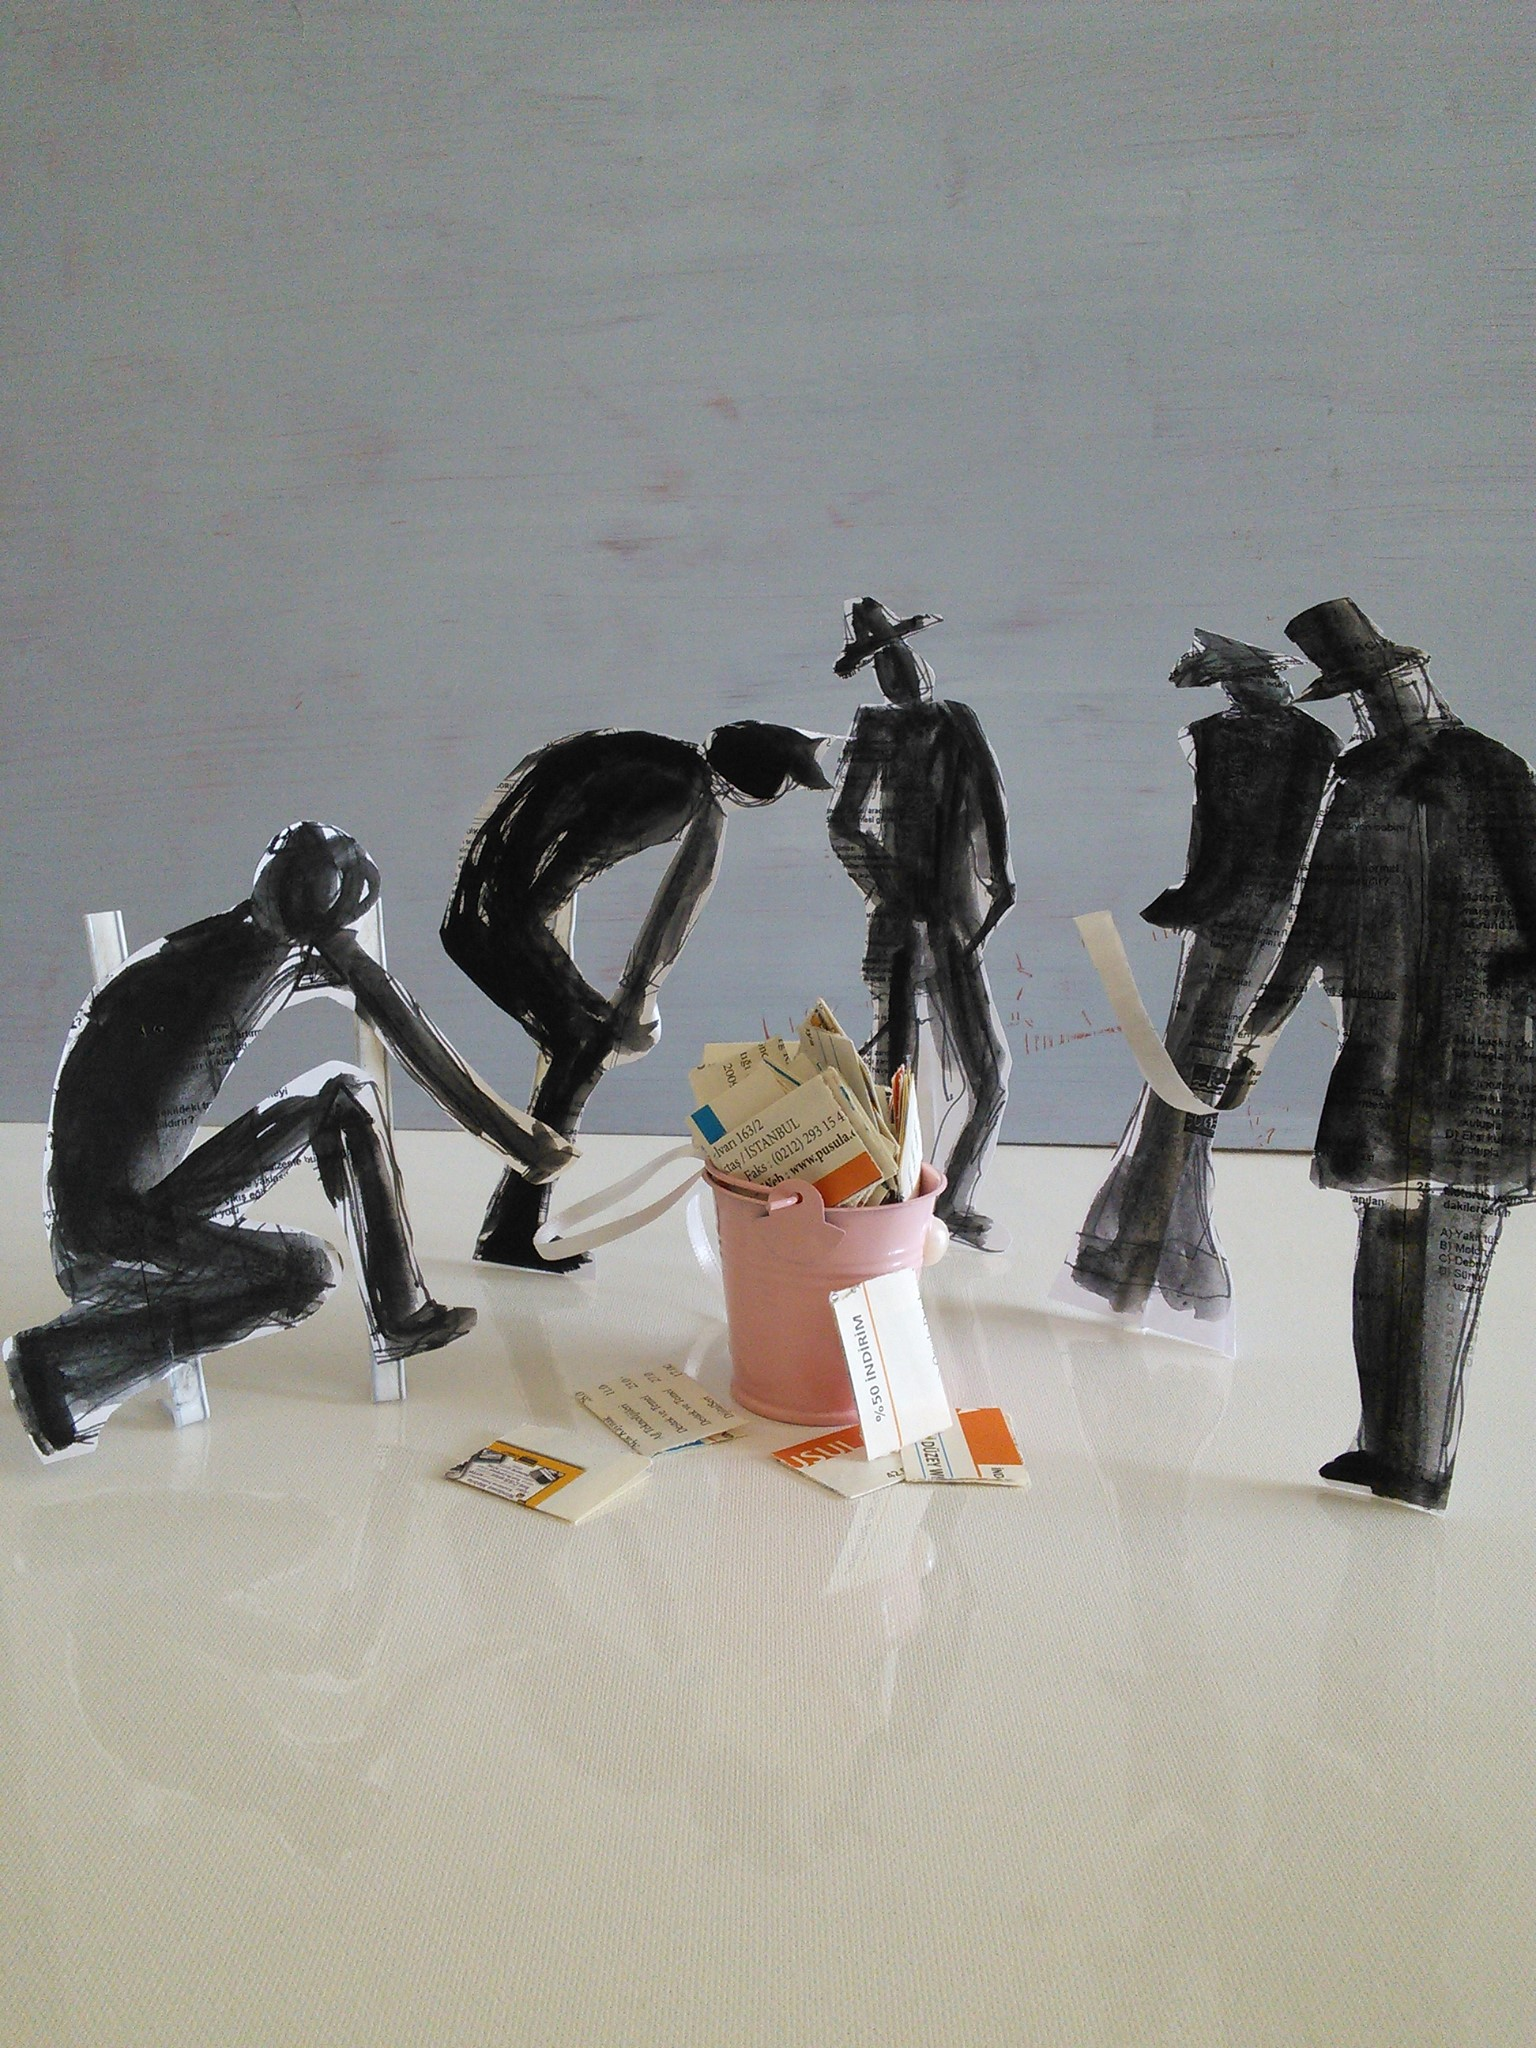
\includegraphics[width=\textwidth]{project_graphics/exhibition2.jpg}
        %\caption{Violin}
        \label{fig:exhibition2}
    \end{subfigure}
    \begin{subfigure}[b]{0.3\textwidth}
        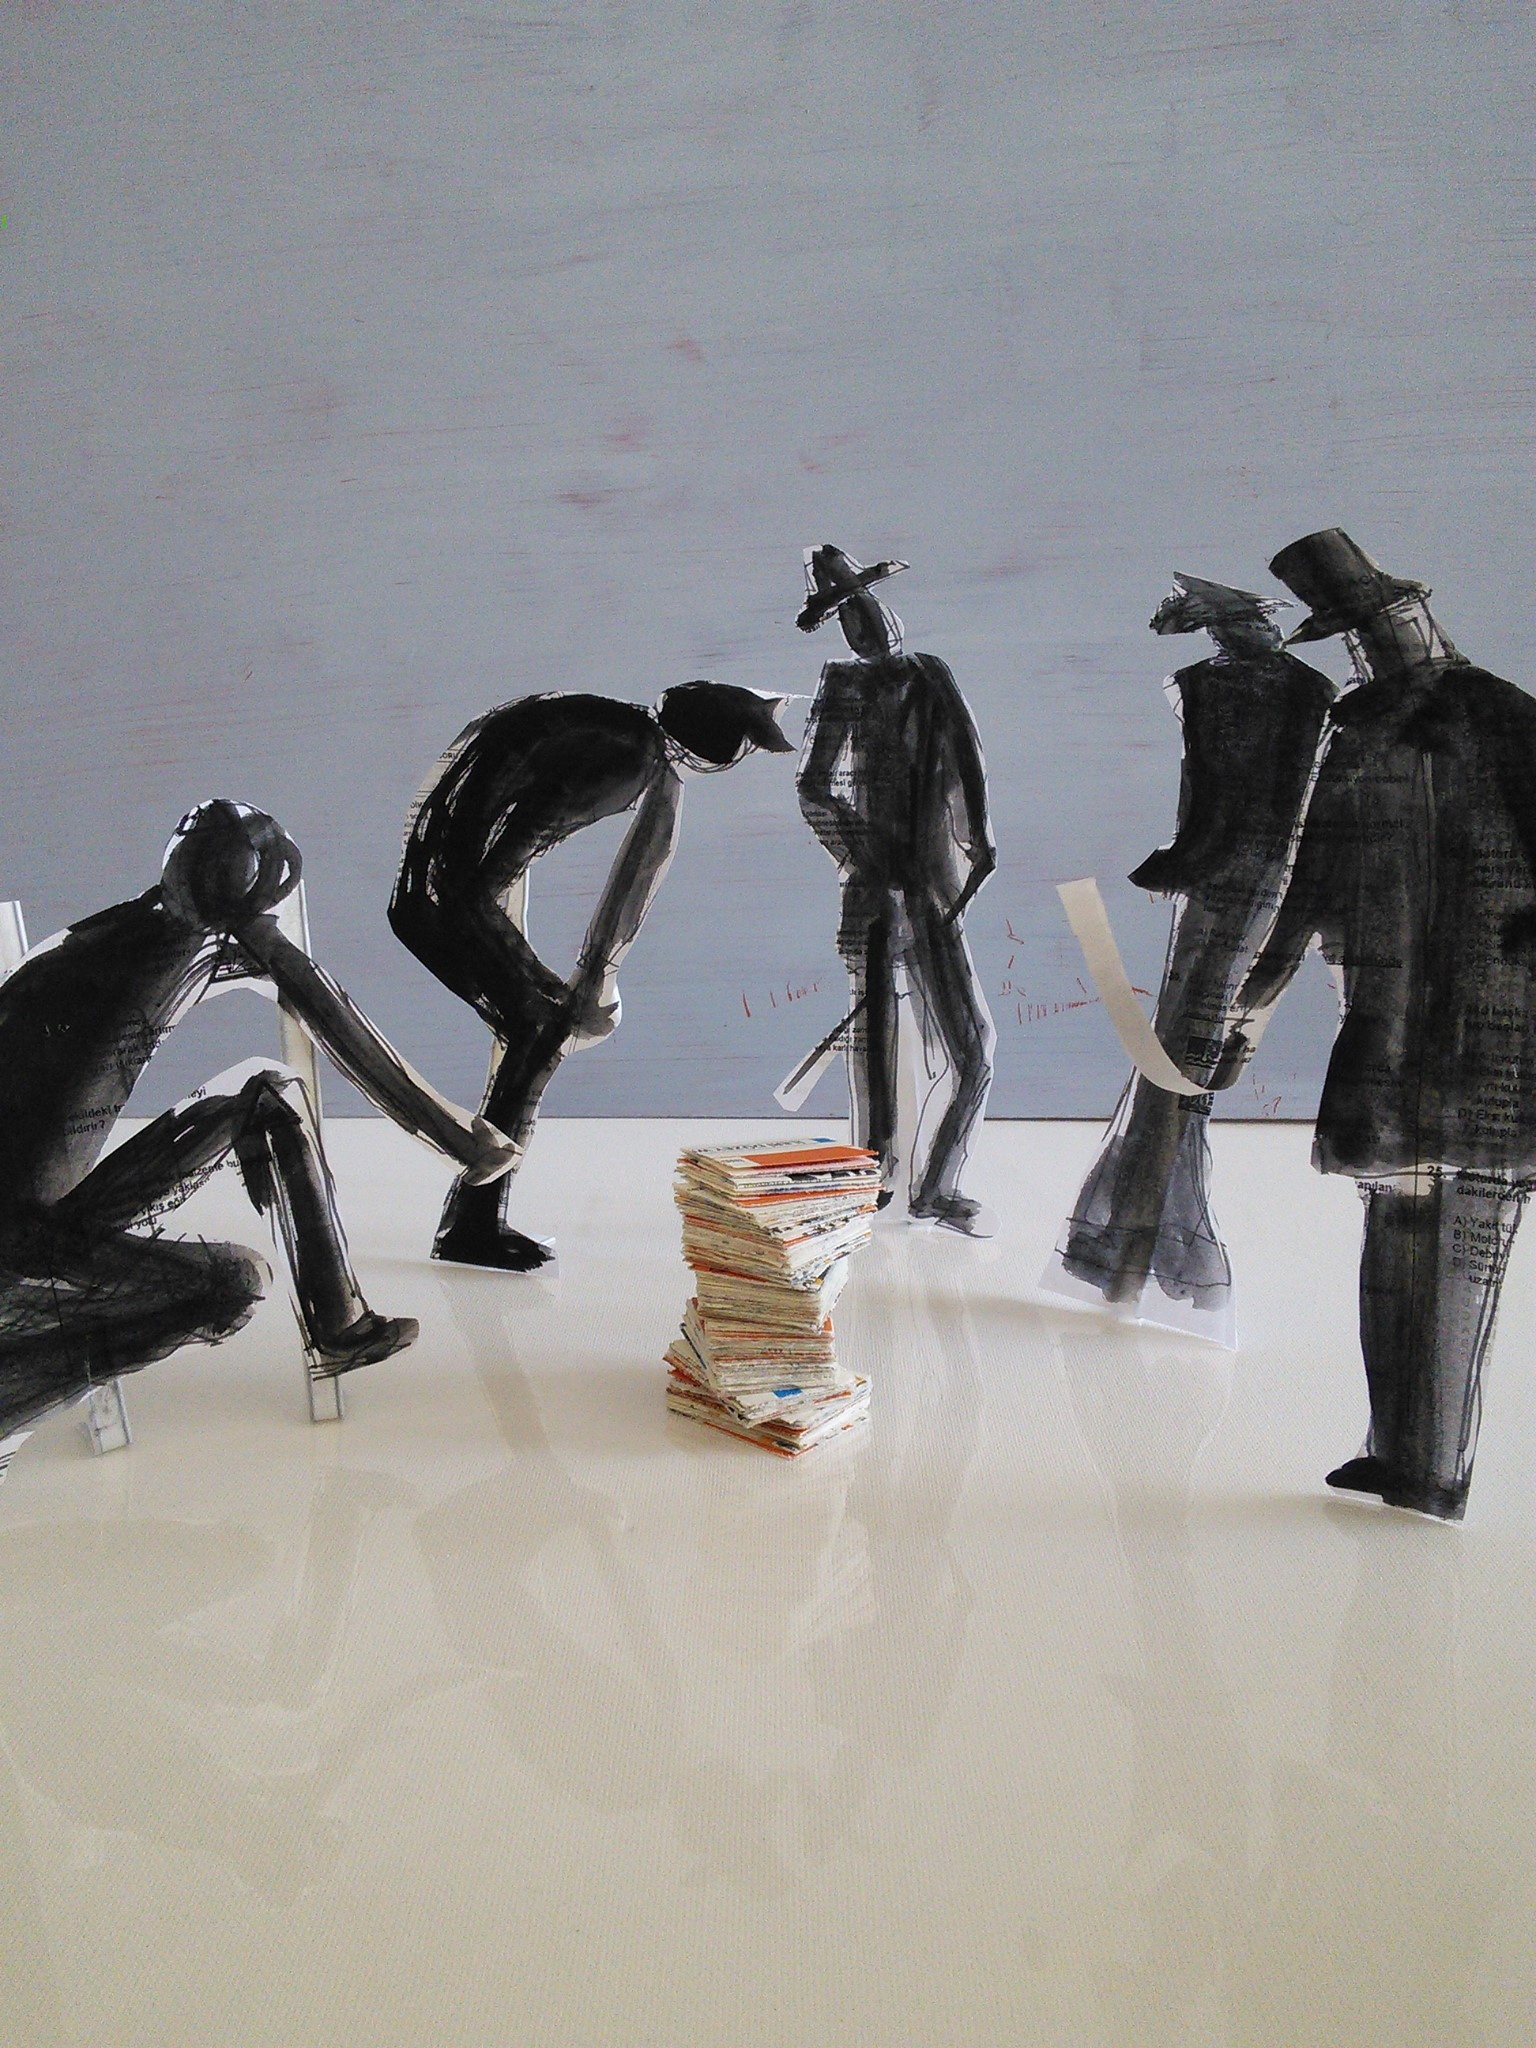
\includegraphics[width=\textwidth]{project_graphics/exhibition3.jpg}
        %\caption{Violin}
        \label{fig:exhibition3}
    \end{subfigure}
    \caption{Installation experiments with models}
    \label{fig:exhibition}
\end{figure}

They were early interpretations and ideas. I imagined an exhibition environment to place notebooks. Different placements were tried. All of them looked like sculpture. I have inserted no special meaning as sculpture to this object an I also I am afraid that people does not close them to the notebooks and look them away. which I do not want.

Aim is to spread the idea by making something useful from trash. Increase diversity, activate (or encourage) people to embrace the trash.

% Bu örnekle insanlara daha fazla yakın olmam gerektiğini gösterdi bana. onların ayaklarına bu proje gitmeliydi. ziyaret ettikleri bir yerde olmalıydım.

% [Why in the public space?] To reach more audience. Actually the audience is out of the art galleries. They are walking in the streets. Putting them to next to people is much more effective. It is not visible and nearly it is hided from society. It is dirty. Removed from the society. There is a effort to hide them away. However in this project it is again showed to the society. Because it is revisited and reclaimed.

% TODO [Why giving away?] Felix Gonzales Torres, Unlimited Editions.
% TODO insanlar bu defterleri alsınlar.





%
%
\section{Parts of project (or final work)}
% TODO la olum bir önceki kısımla bir ilişki kur istersen ha?
The project introduced in this thesis have different parts. Each part support the other. They are connected with each other. Different parts lead different inqueries.

%
%
\subsection{Notebooks}

% TODO notebook hakkında daha fazla şey söylebilmelisin tamam?

Notebooks have been used for different purposes such as drawing, writing and recording, ideas or memoranda by many artists, scientists, and thinkers through the ages. Further same exist for me and people around me. Although the digital alternatives of it paper maintains its place in the community.

Through this project handmade notebooks are produced from discarded paper. They are impure, imperfect and different than usual industrial notebooks. They still carry the traces of previous usage. Every one of them have different stories. Combination of various pieces offer new interpretations of writing.

There are different types of notebooks regarding their color, shape, size and combination. They are simple, imperfect and different than usual industrial notebooks, but more importantly they are from trash. Every one of them has a unique serial and with that serial the (hi)story of it can be viewed.

% Meaning of stories behind the process
There are different stories behind the objects. I try to record their stories (by photography and taking notes) but some of them were not possible. However I still use them in the work because even if I missed their story, with their materiality reveals their history. It still has a history but needs to rewritten. Maybe forgetting all the history maybe creates different notebook.

Every notebook has numbers and with this numbers it can be tracked down when it was produced and which materials are used production of it.

There are notebook series that have a name. Here are the name of notebooks and their story:

\textbf{Puzzle.} Papers inside of the notebooks are cut out from very big and long banner (Figure \ref{fig:Banner_1}). As mentioned previously the objects are bring their history. They are not blank. Heterogen, hiybrid. It can be one of the examples of this argument.

\textbf{09:00 am.} Breakfast time. I think that these packages are used at the morning, very the beginning of the day.

\textbf{12:00 pm.} Burger King pockets from office where I work. Because it is launch time. It is collected at the same time.

\textbf{Friday Night.} (Maybe there can be another option related with traveling, or union). These notebook's pages are collected from restaurant "Varuna Gezgin". We go there to meet some friends after long time. One of them is coming from Australia, the other one is coming from Norway. they are my friends from the university. We united again at varuna gezgin. The place also interesting story. It is a place of travelers. It supports them. and the decoration of that place contains a lot of items collected from different sides of the world. The concept of the place and our meeting perfectly matched. I'm collecting the paper that are under the plates. When we are leaving this place, I ask the guy at the desk, I am making small notebooks and is it possible to exhibit there. I said that is it possible to give them to people. Firstly he asked me that selling them but I said no they are free and part of my thesis project. and later he offered me there are a lot of unused papers. I can give you. they are not used and waiting to be recycling. I took some of the papers, and that papers are part the sheets of these papers.

% Name of the paper can be related with this place and related with the meaning.

% Refer to 9 canlı. Never dies, revives again and again. Because trash moves in the community, even if thrown away can be find another use. Ikinci kez degilde ucuncu kez kullanilan bir sey olursa aslinda onkara dokuz canli demek istiyorum. Gorunus acisindan farkli olmasalar da aslinda isin farkli yanlarini gormek icin faydali olabilirler.

% 9 canlı (cat) / puzzle / bir de dada kelimesi. 9 canlı olmanın kaynağı neresi abi..

% Maybe Later
% Counter Argument:
% People may think and raise the question that none of notebooks is actually my work they belongs to others, others(Starbucks, Burger King) designed it and I am stealing their work. Here there are available different answers to the question. Firstly they are different once they are designed. Turned to different thing. I suggest that them to consider in different context like Duchamp.






%
%
\subsection{Exhibition}
Especially it is the most hard topic in the development of the thesis. To find an appropriate place for the notebooks is great challenge for me.

\textbf{Public space.} The reason why select library is there are small papers to write down the location of books. Libraries are places that things are reused. Books are used by many people. It is place of sharing culture. Books are shared by all the other peoples. Public space. It is place that students from different department use the same place.

Notebooks are places where people frequently visit such as computer desks.

\begin{figure}
    \centering
    \begin{subfigure}[b]{0.47\textwidth}
        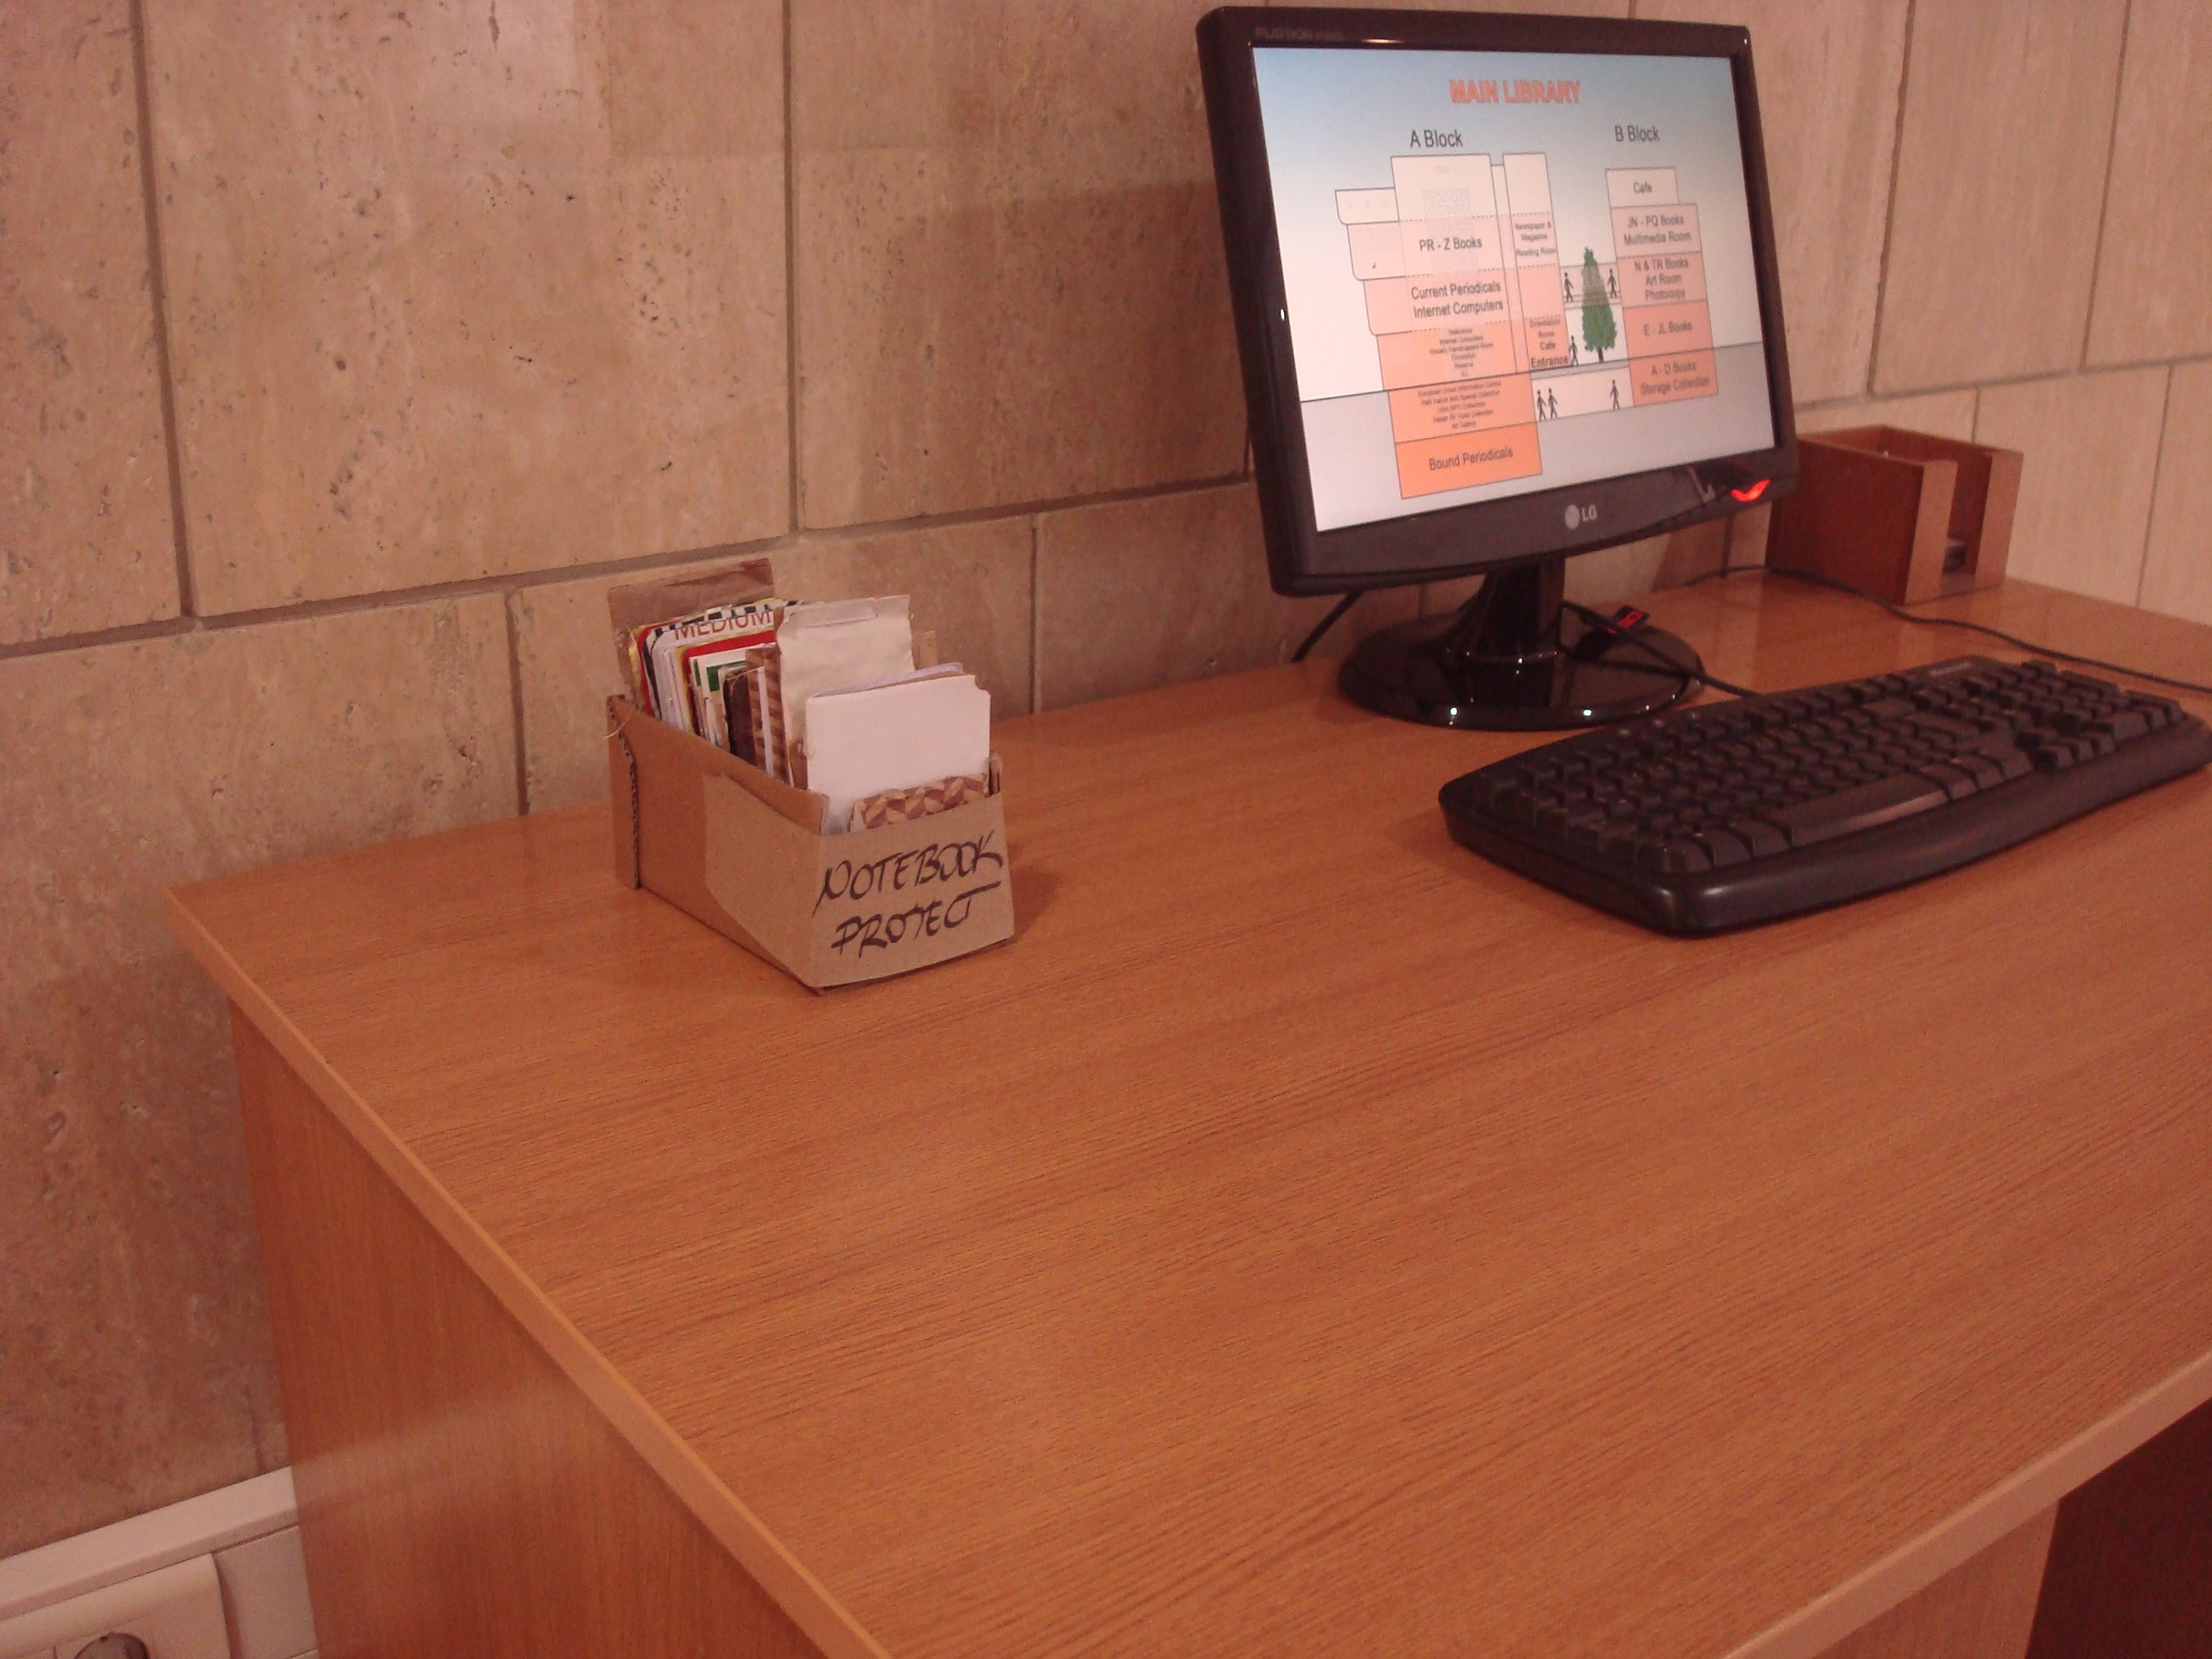
\includegraphics[width=\textwidth]{project_graphics/bilkent1.jpg}
    \end{subfigure}
    \begin{subfigure}[b]{0.47\textwidth}
        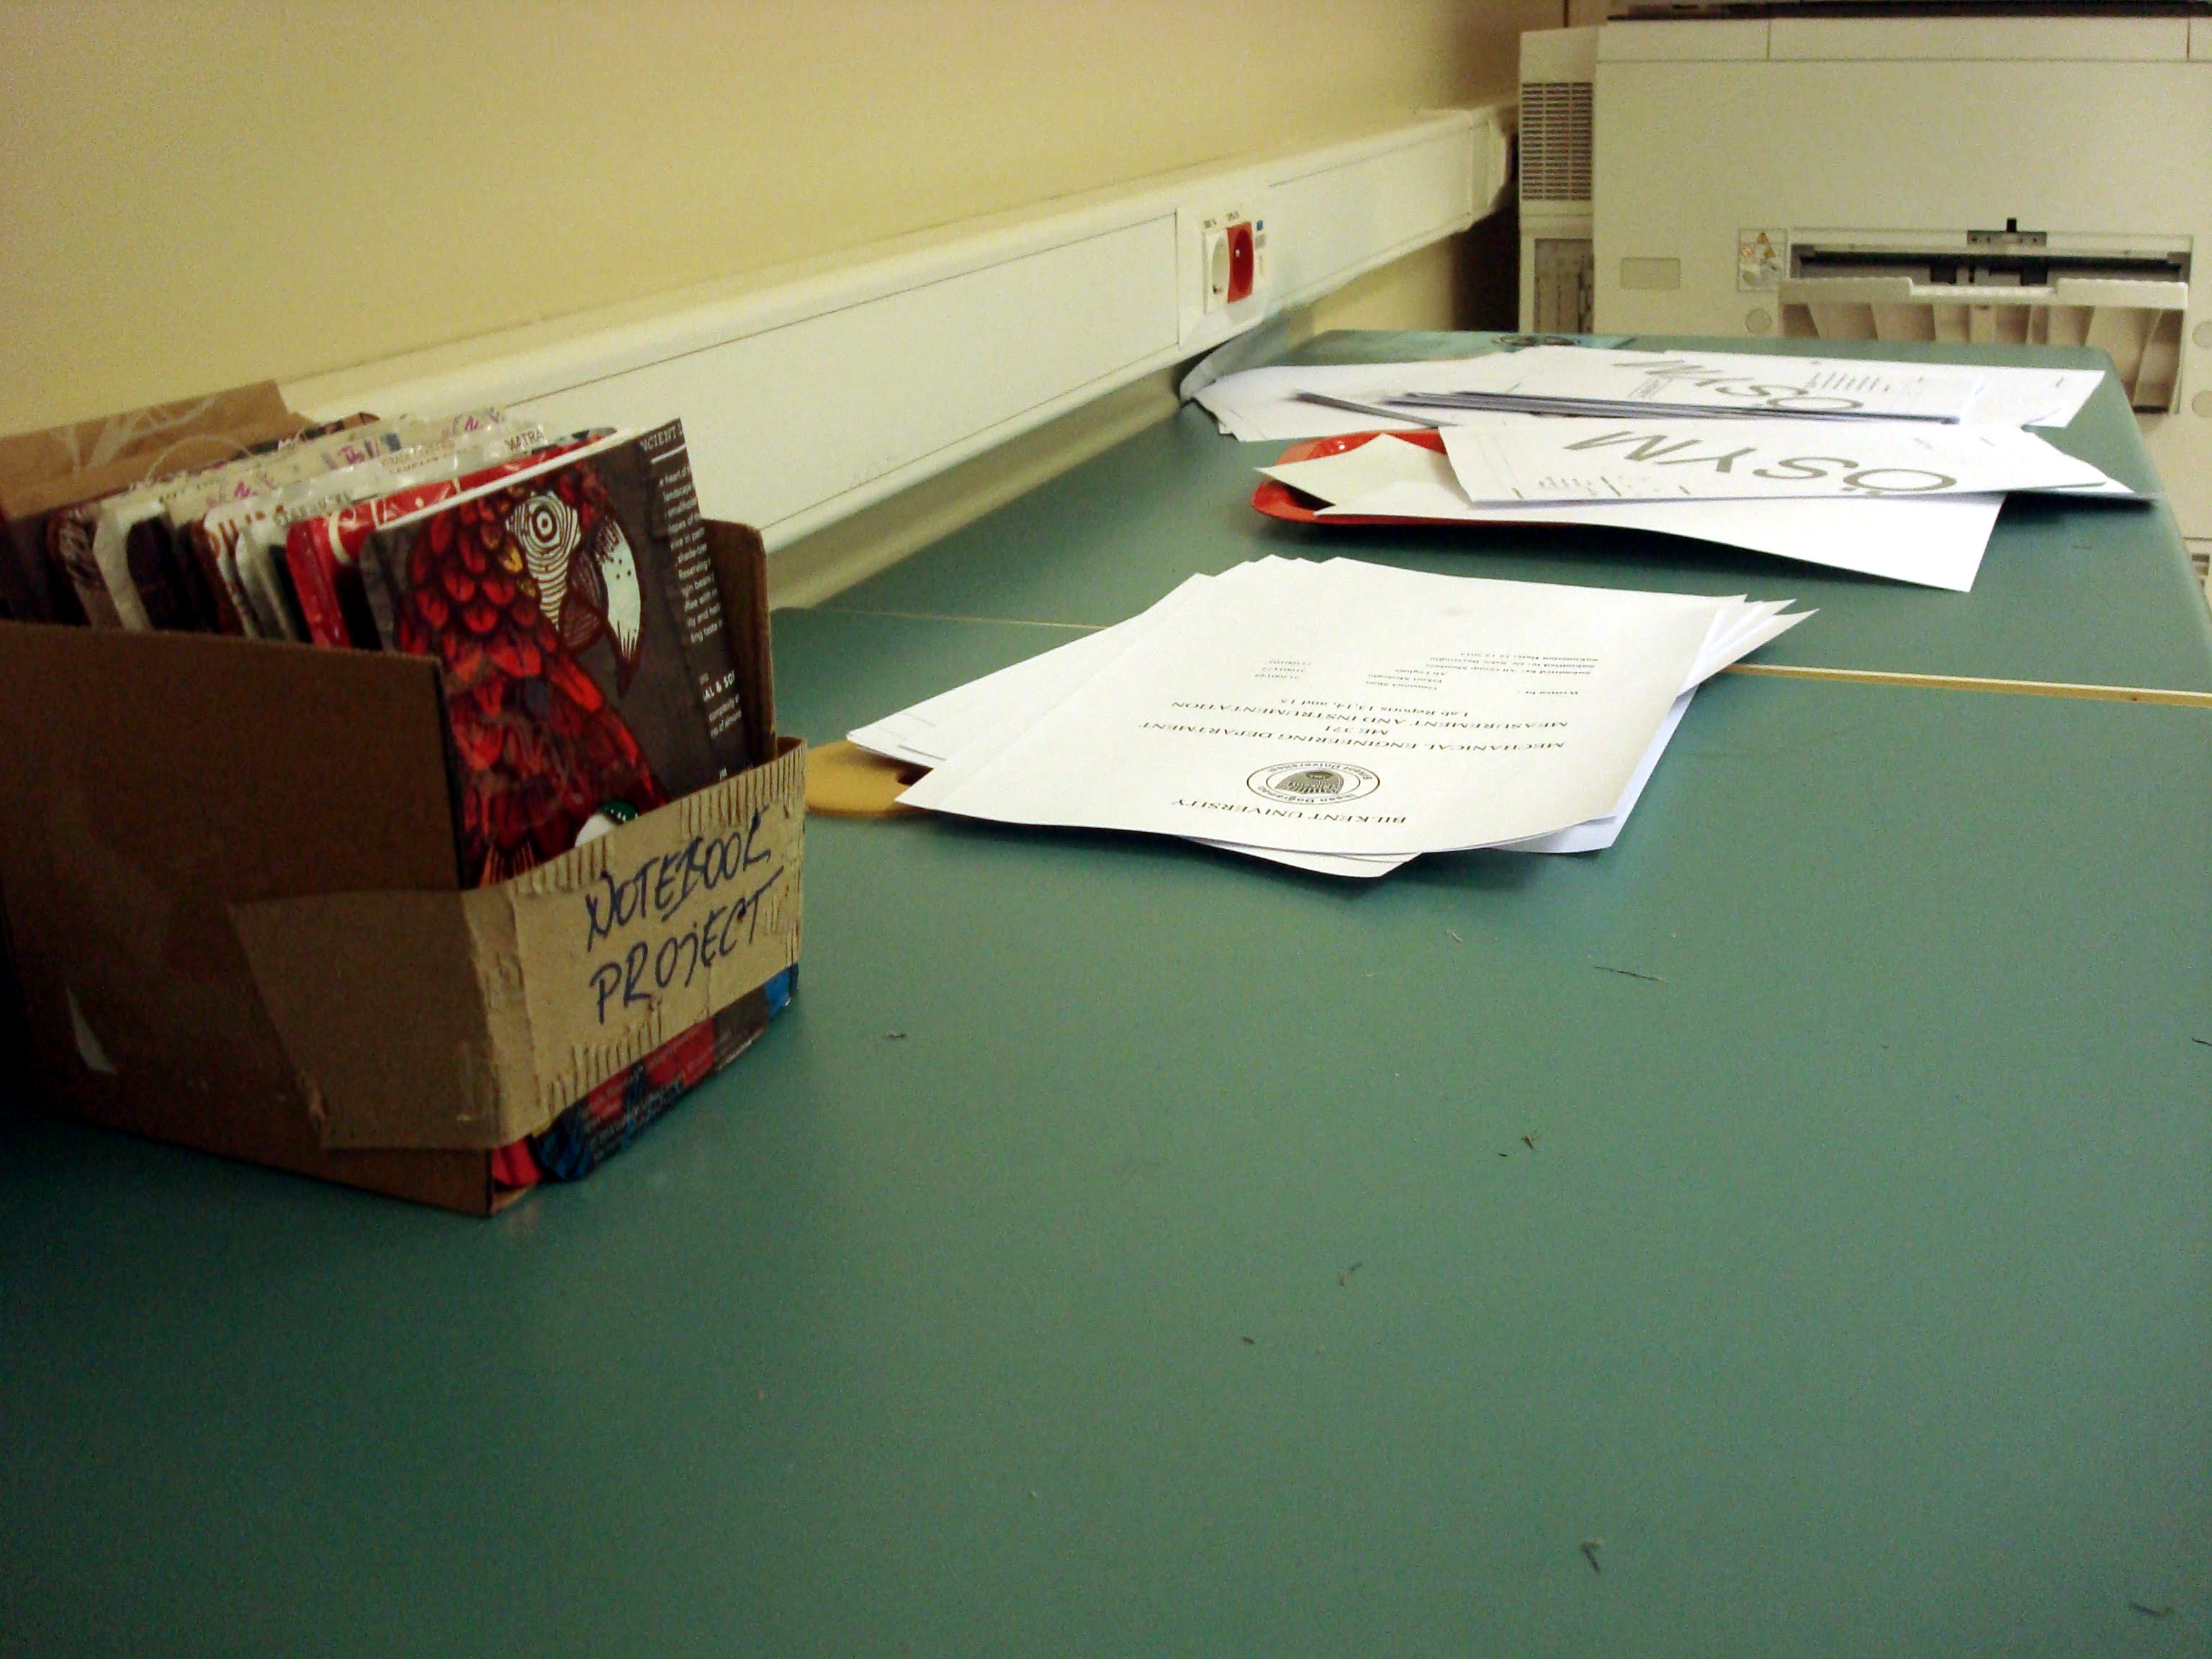
\includegraphics[width=\textwidth]{project_graphics/bilkent2.jpg}
    \end{subfigure}
    \caption{Example placement at Bilkent}
    \label{fig:ExperimentWithPaper}
\end{figure}



% Bilkent, METU, Milli Kütüphane. Buraya nasıl gidilecek. Ama öncelik zaten bilkent kütüphanesinde. ODTÜ sonra geliyor.

% TODO bir çok insanın ortaklaşa kullandığı bir alan. kesişim alanı. bir tanesi de özellikle zaten toplanan yer. insanların karşılaşmalarını istiyorum. karşılaşma noktası.

% Selected places are frequently visited by people. Shared places. 

% TODO  [Yerleştirme fotoğrafları]

Through this project another exhibition alternative is thought. In the notable museums and art galleries there are gift shops that people can buy souvenirs. Often they are mass produced imitations and replicas of well-known artists work embedded various objects such as cover on the notebooks. At this point I image an art space you can buy these types of items freely. In other words alternative to the existing approach this types of gadgets. Another alternative interpretation can be giving away different that the industrial items such as notebooks from trash as in my project. For this type of approach Torun is a great place to show my notebooks and give them away. Torun describe itself as a place for free place for sharing art. Open to everybody. Makes open call to the any artist. There are no security cameras on this gallery therefore no one is watching you at there. This idea shared with Torun and they accepted it. However Torun will opened after 14th of the January currently I just took some photos at there.

\begin{figure}
    \centering
    \begin{subfigure}[b]{0.47\textwidth}
        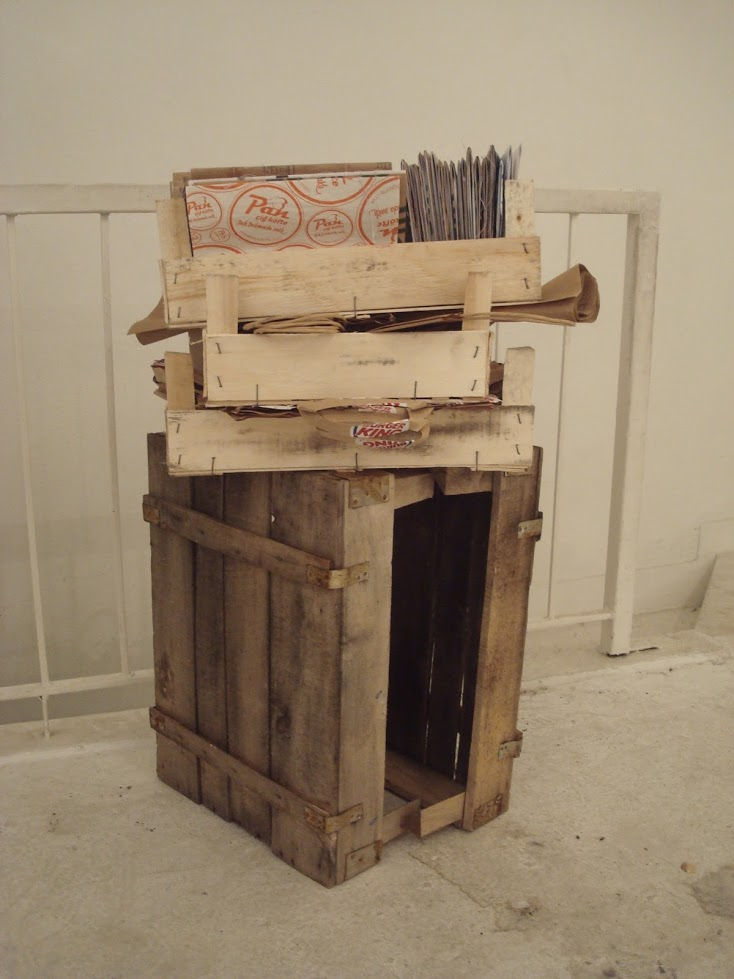
\includegraphics[width=\textwidth]{project_graphics/torun2.jpg}
    \end{subfigure}
    \begin{subfigure}[b]{0.47\textwidth}
        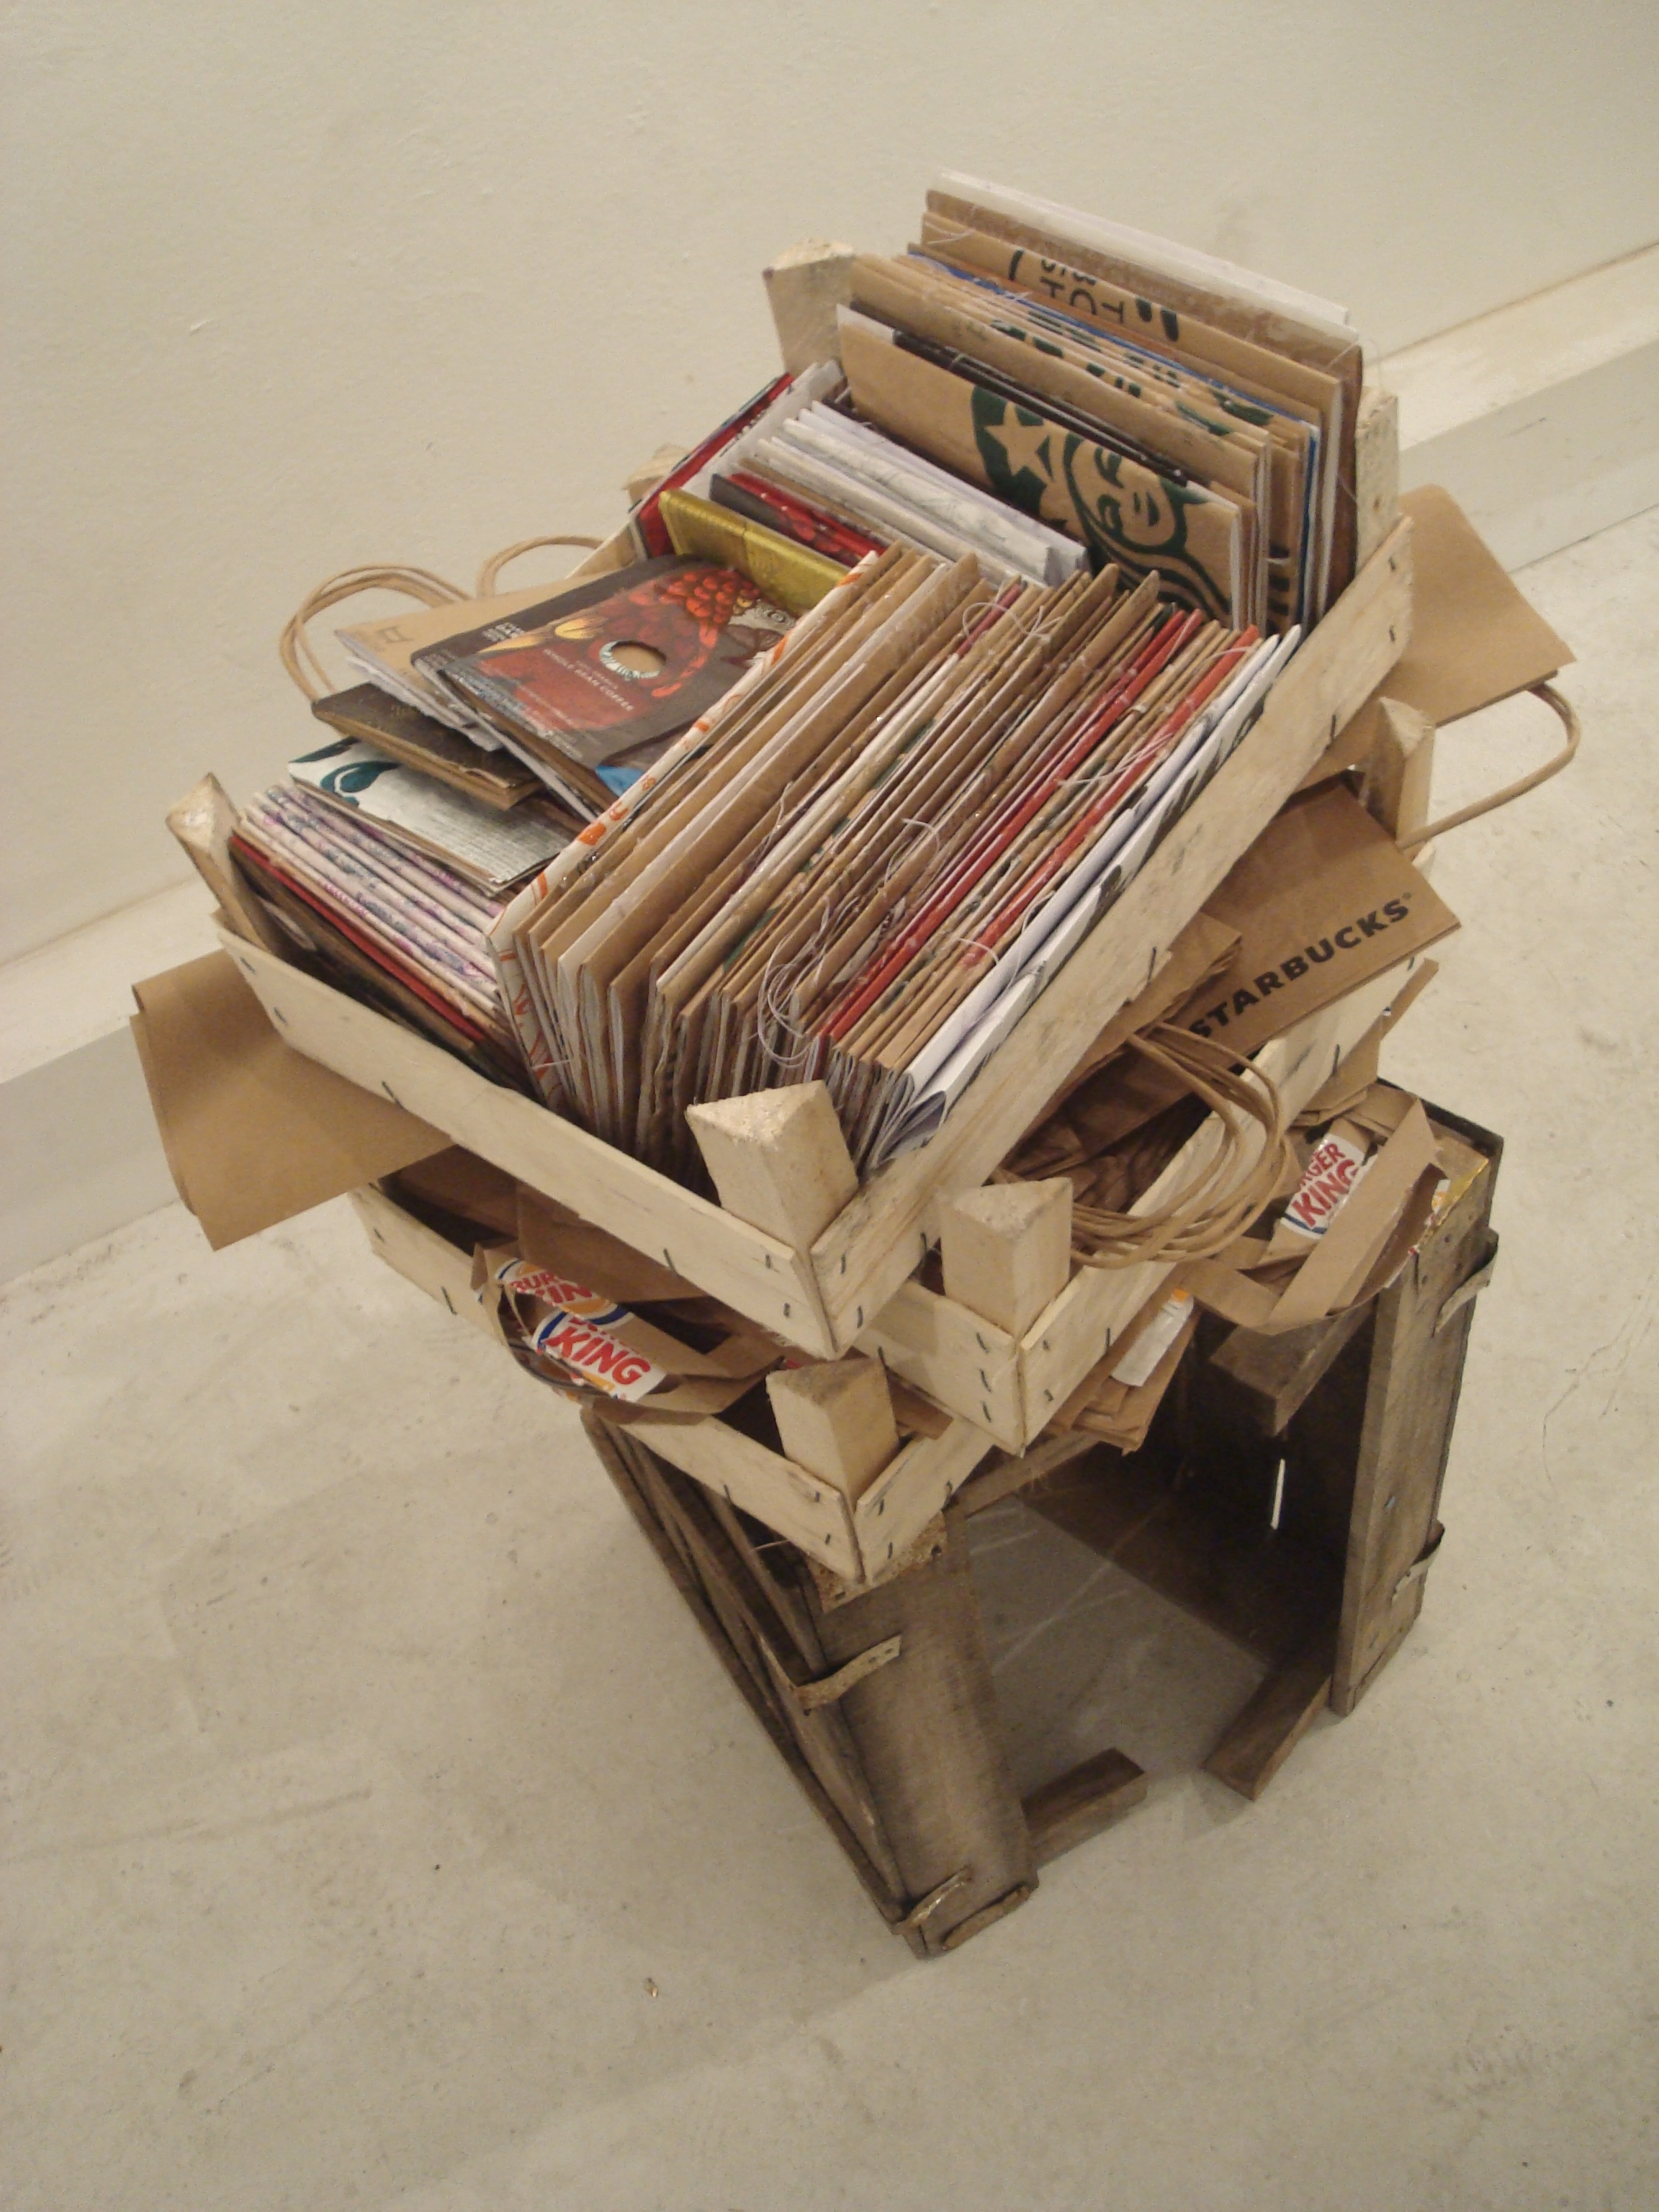
\includegraphics[width=\textwidth]{project_graphics/torun3.jpg}
    \end{subfigure}
    \caption{Example placement at Torun}
    \label{fig:ExperimentWithPaper}
\end{figure}




%
%
\subsection{Website}
As I think that finding a place to the discarded items is one of the main purposes of this project. As it finds a place in people's life again, it also finds another place in the digital space.

Mainly websites displays the (hi)story of notebooks. Further it is a place to track the journey the notebooks. As I claimed that it is not a finished work. Transformation of it does not completed. It always continues. Therefore a website that anyone can reach and share their progress via website  Anyone can later discover how they turned to new things.

As I leave notebooks different places I do not have connection with people who take them. This website also will help to collect/share peoples ideas about the notebooks.

It will contain a section for how notebooks are produced and the story behind it. The purpose is to record the creative process and share with the others. Revealing the process is significant to demystifiying the truth about the project. It makes it more clear that the object used here is actually transformed from something else.

Maybe it can be thought that there are different methods to accomplish recording and sharing the process. In a gallery on a single table or a room it can be succeed. However it like the idea that website can evolve by time as this work evolve in time. I think it matches perfectly. This is not a finished work, it continues and so the website also.

%SketchBook Project is also inspired me a lot especially in terms of website. This project provides a platform to people in order to share their works with other people. It contains lots of works from all over the world. Full of creativity and showcase of richness of people's expressions on the small notebooks. My work can be considered as a sketch book project through trash. Sketches or only creative progress is not the only consideration. You can send your lecture notes.

% [Why website] (database, establishing communication, tracking in time) It was not only that such characteristic was clearly suited for the exploration of human spaces such as home, but it was also that I am comfortably and confidently fluent in coding and web development.

Website can be accessible through the this address http:\\kulu.be\\notebook-project. Domain name kulu.be belongs to me and project placed under a directory of it. Website is coded by me with the common and trusted open source libraries and frameworks. Its code also available at this address. Site is served from GitHub pages which provides free website hosting. Pages are generated by Jekyll which is a static website generator through it some repetitive works are can be easily automatized. 

People can access to images and descriptions of notebooks. All the development process of the project will be revealed in this website. Will contain list of collected materials. 

Into the notebooks a sticker which contains qr code and short description with the address of website is pasted. People can able to reach more information through this reminders. 

\begin{figure}[h!]
  \centering
  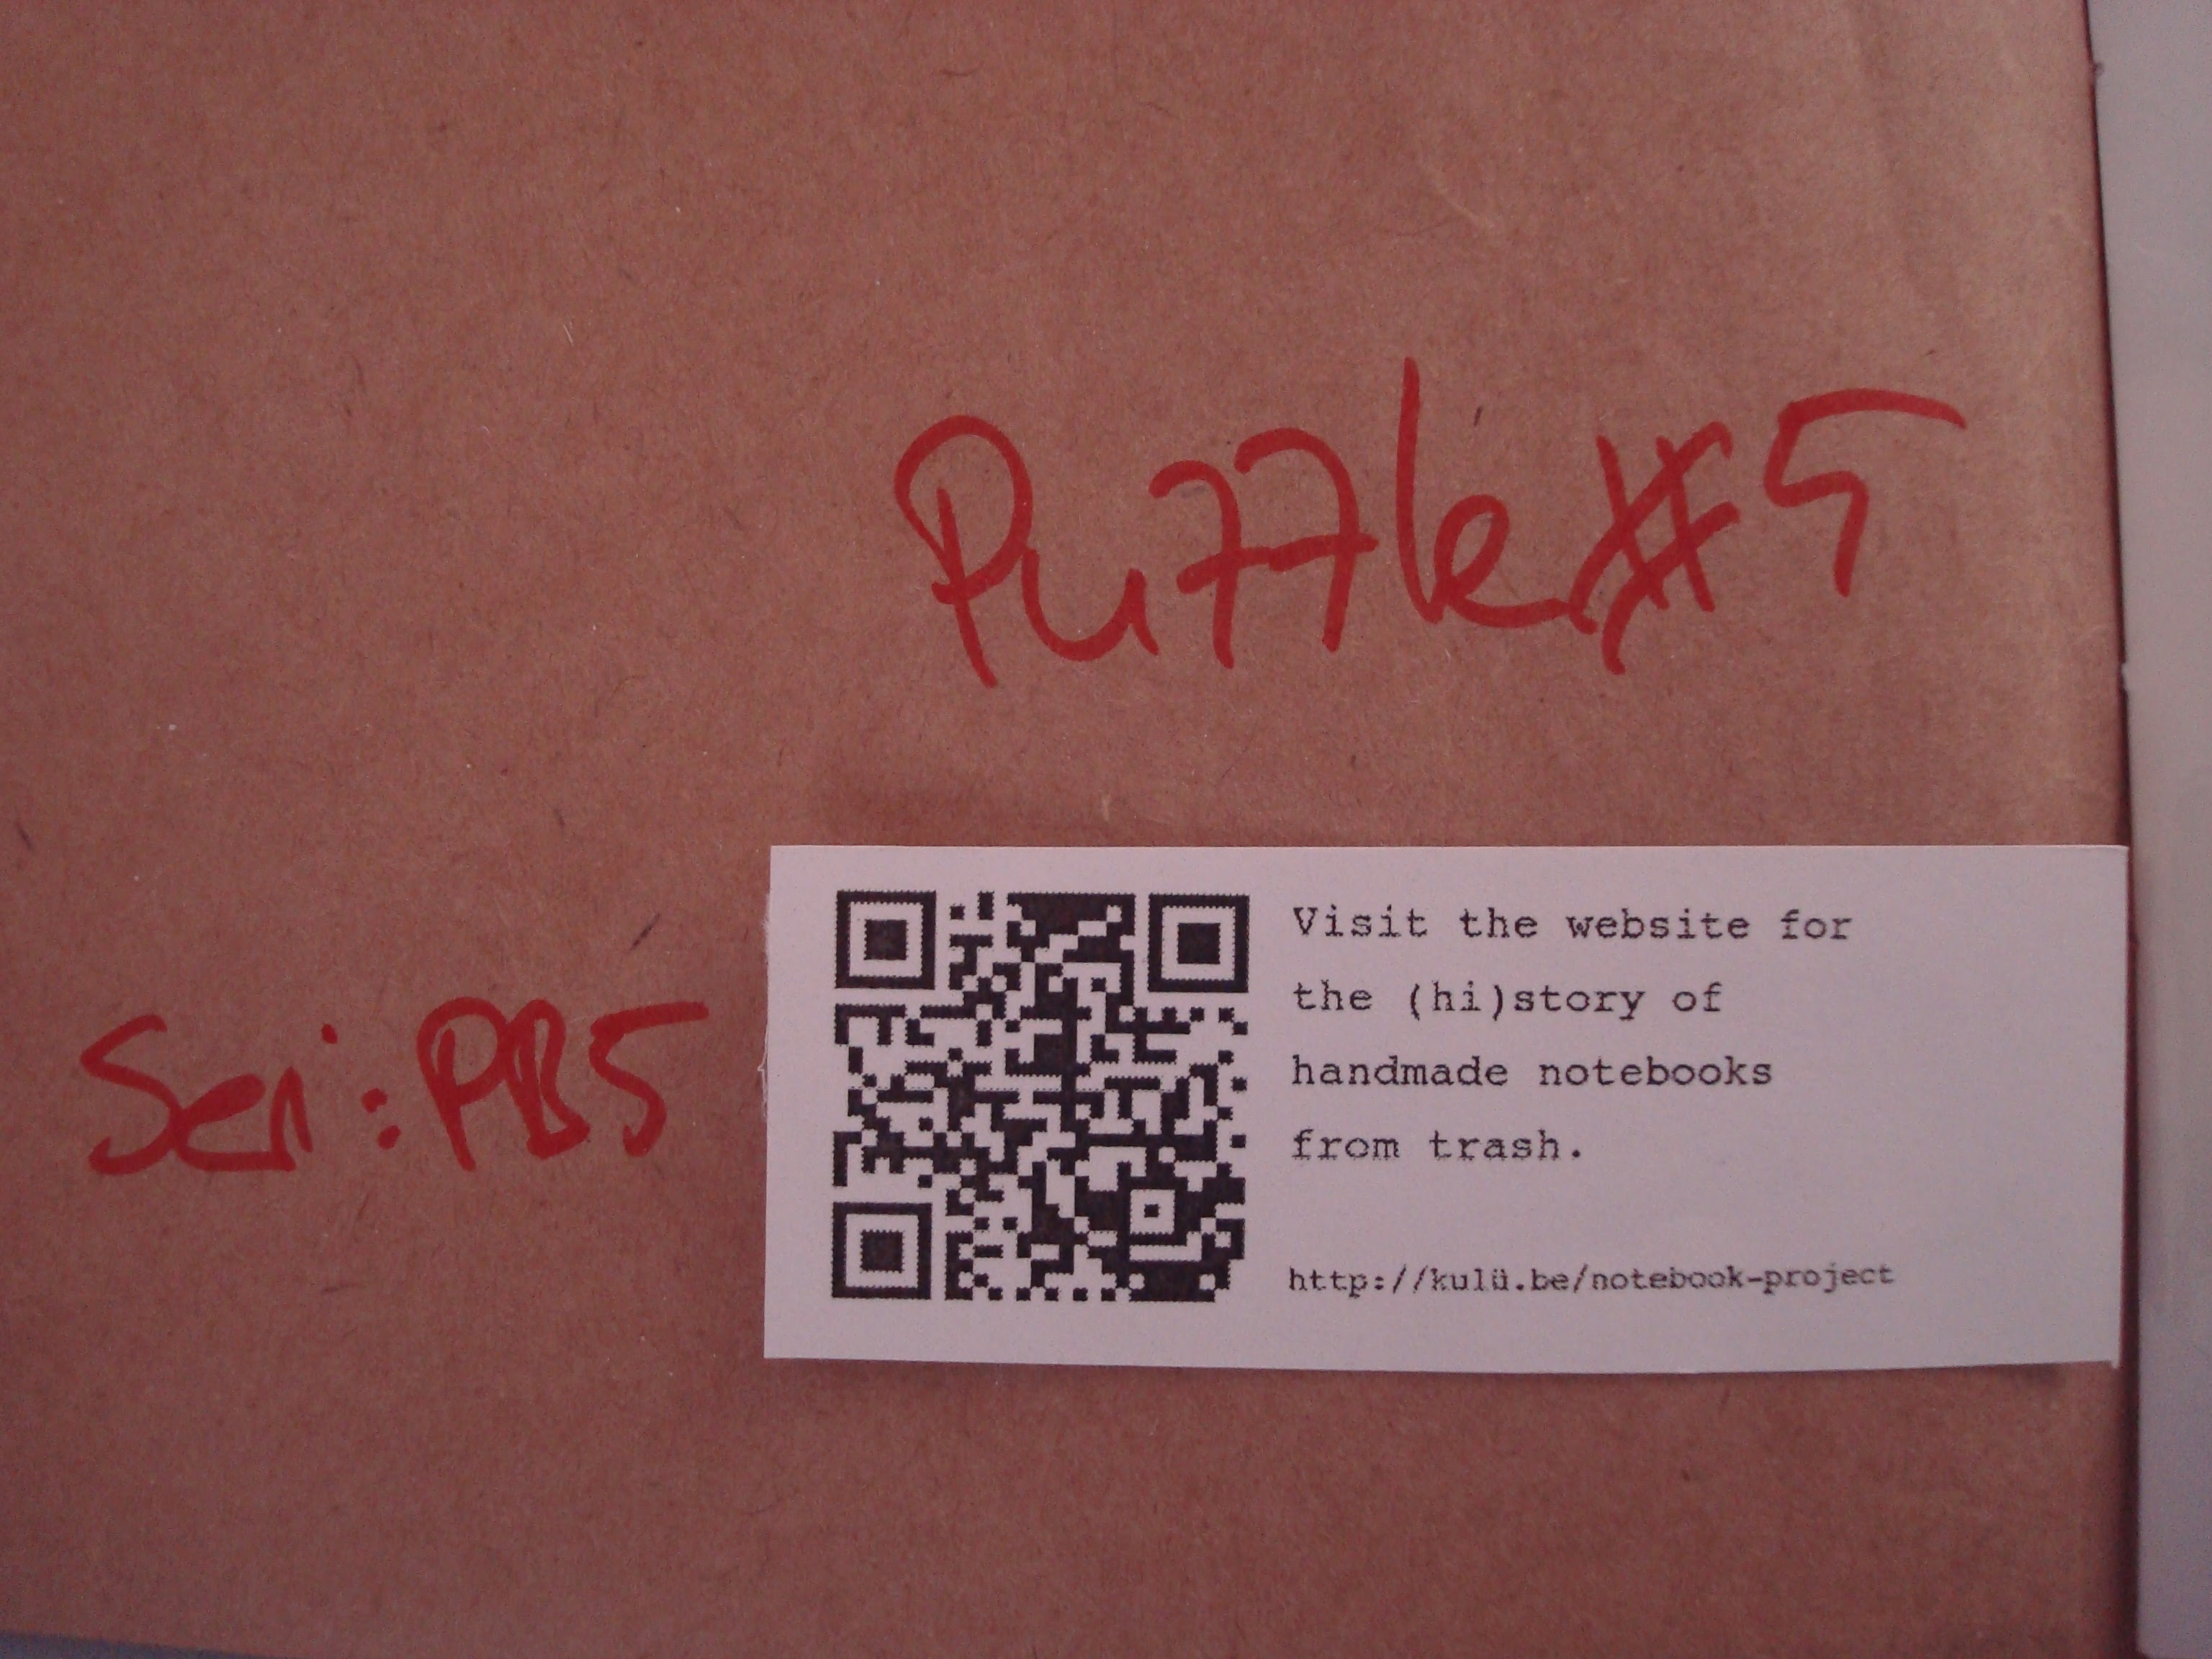
\includegraphics[width=1\textwidth]{project_graphics/qr_serial.jpg}
  \caption{QR Code sample}
  \label{fig:Banner_1}
\end{figure}

Through the website people can be able to subscribe to the newsletter to get updates about the project. People can be able to add their comment to the website. How they are using their notebooks will be showed through it. Website will function as a platform to get into touch with people. From one point of view website can bee seen as a visitors book.

In the future all the discussions and research can be moved to the website that people can reach more information about the subject. This thesis and presentation will also be added to the website. 

All the progress up to now forms the core of the project. However it is not limited with it. The project will be continued after this thesis completed. New features will be added to the website. In the future it is planned that through the website people can be able to request to get notebooks. Thus project becomes more accessible to the other people. Moreover notebooks done by others from trash can be added to the website. Beyond notebooks various objects transformed from trash can find a place in the website.

% MAYBE LATER
% trasnformation practices...
% Notebooklar insanın yanında kolayca taşınabildiği için aslında bir yandan fikri yaymak için ideal. Zaten showing off'un ne kadar önemli olduğu rubbish theoryde söylenmişti.

% MAYBE LATER
% [Standartlar, Dönüştürme seviyesi] endüstriyel standartlar, kaplar ve kağıtlar hep bir şekilde bir birleriyle boyut olarak uyuşuyorlar. İlk başlarda kesip biçmeye daha çok ihitiyaç duyarken zamanla basit katlamalar işimi görmeye başladı. Ne kadar az müdahele bulunursam aslında o kadar çok geldiği yerin özelliklerini o kadar çok temsil ediyordu. Bu da benim hoşuma gidiyordu. Kolaj mantığı işte abi. Ne kadar çok değiştirmek dönüştürmek istiyorsun. Burda şöyle bir durum var. çöpleri hiç tanınmayacak bir hale de getirebilirsin. Bu şekilde kimse onların farkına bile varmaz. Ya da neredeyse olduğu gibi kullanırsın. Yani uygulanan dönüştürmenin derecesi çok önemli burada...
